% =====================================================================
%  ESP32-S3 Production Firmware — Corrected MQTT Sequence (EMQX best practice)
%  ETERNITY / ONEOPS Platform — companion to the Unified Technical Spec
%
%  Build:  pdflatex esp32-firmware-sequence.tex   (run twice)
%  Pure TikZ — no external sequence-diagram package required.
% =====================================================================
\documentclass[11pt,a4paper]{article}

\usepackage[utf8]{inputenc}
\usepackage[T1]{fontenc}
\usepackage[margin=2.2cm]{geometry}
\usepackage{xcolor}
\usepackage{amssymb}
\usepackage{booktabs}
\usepackage{array}
\usepackage{tabularx}
\usepackage{enumitem}
\usepackage{graphicx}
\usepackage{caption}
\usepackage{float}
\usepackage{tikz}
\usetikzlibrary{arrows.meta,calc,positioning,backgrounds,fit,shapes.misc}
\usetikzlibrary{shapes.geometric,chains}
\usepackage{listings}

% extra palette for hardware / firmware diagrams
\definecolor{hwCol}{HTML}{DAE8FC}\definecolor{hwEdge}{HTML}{6C8EBF}
\definecolor{drvCol}{HTML}{D5E8D4}\definecolor{drvEdge}{HTML}{82B366}
\definecolor{profCol}{HTML}{FFE6CC}\definecolor{profEdge}{HTML}{D79B00}
\definecolor{appCol}{HTML}{B0E3E6}\definecolor{appEdge}{HTML}{0E8088}
\definecolor{cloudCol}{HTML}{E1D5E7}\definecolor{cloudEdge}{HTML}{9673A6}
\definecolor{crossCol}{HTML}{F8CECC}\definecolor{crossEdge}{HTML}{B85450}
\definecolor{sysCol}{HTML}{FFF2CC}\definecolor{sysEdge}{HTML}{D6B656}
\definecolor{halCol}{HTML}{F0F0F0}\definecolor{halEdge}{HTML}{8C8C8C}

\tikzset{
  layer/.style n args={3}{draw=#2, fill=#1, rounded corners=2pt, align=center,
        font=\scriptsize, minimum height=0.9cm, text width=#3},
  sidebar/.style n args={2}{draw=#2, fill=#1, rounded corners=2pt, align=center,
        font=\scriptsize, text width=1.9cm},
  periph/.style n args={2}{draw=#2, fill=#1, rounded corners=3pt, align=center,
        font=\scriptsize, inner sep=3pt, minimum width=2.9cm, minimum height=0.8cm},
  fproc/.style={draw=hwEdge, fill=hwCol, rounded corners=3pt, align=center,
        font=\scriptsize, inner sep=3pt, minimum height=0.7cm, text width=3.4cm},
  fdec/.style={draw=profEdge, fill=profCol, diamond, aspect=2.2, align=center,
        font=\scriptsize, inner sep=1pt},
  fterm/.style={draw=sysEdge, fill=sysCol, rounded corners=12pt, align=center,
        font=\scriptsize\bfseries, inner sep=3pt, text width=3.2cm},
  fsafe/.style={draw=crossEdge, fill=crossCol, rounded corners=3pt, align=center,
        font=\scriptsize, inner sep=3pt, text width=3.4cm},
  fback/.style={draw=sysEdge, fill=sysCol, rounded corners=3pt, align=center,
        font=\scriptsize, inner sep=3pt, text width=3.4cm},
  stnode/.style n args={2}{draw=#2, fill=#1, rounded corners=7pt, align=center,
        font=\scriptsize, inner sep=4pt, minimum width=2.7cm, line width=0.8pt},
  flow/.style={-{Stealth[length=5pt]}, font=\tiny, align=center, line width=0.6pt},
  flowd/.style={-{Stealth[length=5pt]}, densely dashed, font=\tiny, align=center, line width=0.6pt},
  elab/.style={font=\tiny, fill=white, inner sep=1pt, align=center},
}

\lstdefinestyle{js}{basicstyle=\ttfamily\scriptsize, breaklines=true, frame=single,
  framesep=4pt, columns=fullflexible, keepspaces=true, showstringspaces=false,
  backgroundcolor=\color{noteCol!35}, xleftmargin=2pt, xrightmargin=2pt}

% ---------------------------------------------------------------------
%  Palette
% ---------------------------------------------------------------------
\definecolor{devCol}{HTML}{2E7D32}   % ESP32 device   (green)
\definecolor{brkCol}{HTML}{6A1B9A}   % EMQX broker    (purple)
\definecolor{svcCol}{HTML}{1565C0}   % services       (blue)
\definecolor{dbCol}{HTML}{00838F}    % datastore      (teal)
\definecolor{otaCol}{HTML}{EF6C00}   % OTA / artefact (orange)
\definecolor{usrCol}{HTML}{C62828}   % operator       (red)
\definecolor{bandCol}{HTML}{ECEFF4}  % phase band
\definecolor{noteCol}{HTML}{FFF8E1}  % note fill
\definecolor{noteEdge}{HTML}{F9A825}

% ---------------------------------------------------------------------
%  Sequence-diagram engine (auto-advancing vertical cursor \YY)
% ---------------------------------------------------------------------
\newcommand{\msgstep}{0.70}
\newcommand{\seqreset}{\xdef\YY{-1.30}}
\newcommand{\adv}{\pgfmathsetmacro{\tmp}{\YY-\msgstep}\xdef\YY{\tmp}}
\newcommand{\gap}{\pgfmathsetmacro{\tmp}{\YY-0.35}\xdef\YY{\tmp}}

\tikzset{
  head/.style={draw, rounded corners=2pt, minimum width=2.05cm, minimum height=0.66cm,
               font=\footnotesize\bfseries, text=white, align=center},
  lifeline/.style={densely dashed, gray!60, line width=0.5pt},
  msg/.style={-{Stealth[length=5pt]}, line width=0.7pt},          % control packet / sync call
  evt/.style={-{Stealth[length=5pt]}, densely dashed, line width=0.7pt, brkCol}, % broker delivery / async event
  ret/.style={-{Triangle[open,length=5pt]}, densely dotted, gray, line width=0.6pt}, % return
  mlbl/.style={midway, above, font=\scriptsize, inner sep=1.4pt, align=center},
  mlblb/.style={midway, below, font=\scriptsize, inner sep=1.4pt, align=center},
  notestyle/.style={draw=noteEdge, fill=noteCol, rounded corners=1pt, font=\scriptsize,
                    align=left, inner sep=3pt, text width=#1},
  band/.style={fill=bandCol, draw=gray!40, rounded corners=2pt, font=\footnotesize\bfseries\itshape,
               text=black!75, minimum height=0.5cm, align=center},
}

% solid message:  \mO{fromX}{toX}{label}
\newcommand{\mO}[3]{\draw[msg] (#1,\YY) -- (#2,\YY) node[mlbl]{#3};\adv}
% solid message, label below (for tight return-direction lines)
\newcommand{\mOb}[3]{\draw[msg] (#1,\YY) -- (#2,\YY) node[mlblb]{#3};\adv}
% async broker delivery / event
\newcommand{\mA}[3]{\draw[evt] (#1,\YY) -- (#2,\YY) node[mlbl,text=brkCol]{#3};\adv}
% return / response
\newcommand{\mR}[3]{\draw[ret] (#1,\YY) -- (#2,\YY) node[mlbl,text=gray]{#3};\adv}
% self action:  \mS{X}{label}
\newcommand{\mS}[2]{%
  \draw[msg] (#1,\YY) -- ++(0.55,0) -- ++(0,-0.26) -- ++(-0.55,0);
  \node[anchor=west,font=\scriptsize,inner sep=1.4pt] at ([xshift=17pt,yshift=-4pt]#1,\YY){#2};
  \pgfmathsetmacro{\tmp}{\YY-0.82}\xdef\YY{\tmp}}
% note anchored at x:  \note{x}{width}{text}
\newcommand{\note}[3]{\node[notestyle=#2] at (#1,\YY){#3};\adv}
% full-width phase band centred at \xmid:  \phase{text}
\newcommand{\phase}[1]{\gap\node[band,minimum width=\bandw] at (\xmid,\YY){#1};\adv}

\newcommand{\seqtitle}[1]{\textbf{#1}}

% =====================================================================
\begin{document}

\begin{center}
  {\LARGE\bfseries ESP32-S3 IoT Platform}\\[2pt]
  {\large Unified Firmware \& Hardware Specification}\\[4pt]
  {\normalsize One firmware for three products — bloodBOX \(\cdot\) refrigeDataLogger \(\cdot\) transformersMonitoring}\\[6pt]
  {\small ETERNITY\,/\,ONEOPS Platform \(\cdot\) consolidates the MQTT contract, PCB function map and firmware concept}\\[2pt]
  {\small\itshape Revised 2026-06-10}
\end{center}

\vspace{4pt}\hrule\vspace{6pt}

\noindent\textbf{Document map.}\;
\textbf{Part~I} — cloud interface \& MQTT/EMQX contract (\S1--\S9).\quad
\textbf{Part~II} — hardware: ESP32-S3 PCB function map, offline timekeeping (\S10--\S11).\quad
\textbf{Part~III} — firmware concept design: architecture, boot, runtime, link FSM, diagnostics,
LoRaWAN integration, EOL manufacturing, partition table, transport hysteresis (\S12--\S21).
\\[2pt]
Editable diagram sources live alongside this PDF as draw.io files
(\texttt{esp32-pcb-functions.drawio}, \texttt{esp32-firmware-concept.drawio}); every figure here
is redrawn natively so the PDF is self-contained.

\vspace{8pt}\hrule\vspace{8pt}

\part*{Part I\quad Cloud interface \& MQTT contract}
\addcontentsline{toc}{part}{Part I — Cloud interface \& MQTT contract}

\section*{1\quad Scope and what was corrected}
The specification's end-to-end sequence (\S5.6/\S5.7) begins at \texttt{publish reading}
and treats the broker as a dumb pipe. That hides the parts of the firmware contract that
actually decide field reliability: \emph{how the device authenticates, how presence is
tracked, how sessions and commands survive a flaky link, and how firmware is delivered
safely}. This document redraws the lifecycle of a single production device against
\textbf{EMQX} broker semantics (MQTT~5.0) and marks every correction.

\begin{center}
\renewcommand{\arraystretch}{1.28}
\small
\begin{tabularx}{\textwidth}{@{}p{3.0cm} p{4.6cm} X@{}}
\toprule
\textbf{Area} & \textbf{Original spec} & \textbf{Corrected — EMQX best practice} \\
\midrule
Transport \& auth & shared / implicit; ``returns mTLS cert'' but no handshake shown &
  one-time factory \emph{bootstrap} token over server-auth TLS, immediately rotated to
  \textbf{per-device X.509 client certificate}; steady state is \textbf{mutual TLS 1.3}
  verified by EMQX. \\
Client identity & ``initial \texttt{device\_id}'' &
  stable, unique \texttt{mqtt\_client\_id} bound to the certificate CN; duplicate-ID
  takeover rejected. \\
Authorization & not stated &
  EMQX \textbf{ACL}: a device may only publish/subscribe under
  \texttt{devices/\{id\}/\#} and \texttt{sensors/\{sid\}/raw}; cross-device spoofing denied. \\
Session & not stated &
  MQTT~5.0 \texttt{clean\_start=0} + \textbf{Session-Expiry}, so QoS~1 commands queued
  during a brief drop are redelivered on reconnect. \\
Presence (LWT) & \texttt{status} is ``LWT topic'', retain unspecified &
  Will published \textbf{QoS~1, retain=1}; matching \textbf{birth} message on (re)connect
  clears it, so late subscribers always read correct state. \\
Config delivery & plain publish &
  \texttt{devices/\{id\}/config} published \textbf{retain=1, QoS~1} $\Rightarrow$ device
  gets current config the instant it subscribes. \\
Heartbeat & QoS~0, retain=0 \checkmark &
  kept QoS~0; \texttt{keepalive=60\,s}, EMQX dead-peer detection at $1.5\times$ keepalive. \\
Sensor reading & QoS~1, retain=0 \checkmark &
  kept QoS~1 (PUBACK); ingest consumes via an EMQX \textbf{shared subscription}
  (\texttt{\$share/ingest/\dots}) for horizontal scale + back-pressure. \\
OTA & ``upgrade to 1.4.2 from \texttt{artefact\_uri}'' &
  \textbf{signed} artefact (SHA-256 + secure-boot), \textbf{A/B} partition, out-of-band
  HTTPS fetch, \texttt{ota/progress} telemetry, \textbf{automatic rollback}, audit row in
  \texttt{device\_firmware\_history}. \\
Abuse control & none &
  EMQX \textbf{flapping detection} + per-client message/bandwidth rate limits. \\
\bottomrule
\end{tabularx}
\end{center}

\paragraph{Legend.}
\tikz[baseline=-0.5ex]{\draw[msg] (0,0)--(0.7,0);} solid = MQTT control packet / synchronous call\quad
\tikz[baseline=-0.5ex]{\draw[evt] (0,0)--(0.7,0);} dashed = broker delivery / asynchronous event\quad
\tikz[baseline=-0.5ex]{\draw[ret] (0,0)--(0.7,0);} dotted = return / acknowledgement.

% =====================================================================
\newpage
\section*{2\quad Phase A — Zero-touch provisioning \& secure session bring-up}

\begin{figure}[H]
\centering
\resizebox{\textwidth}{!}{%
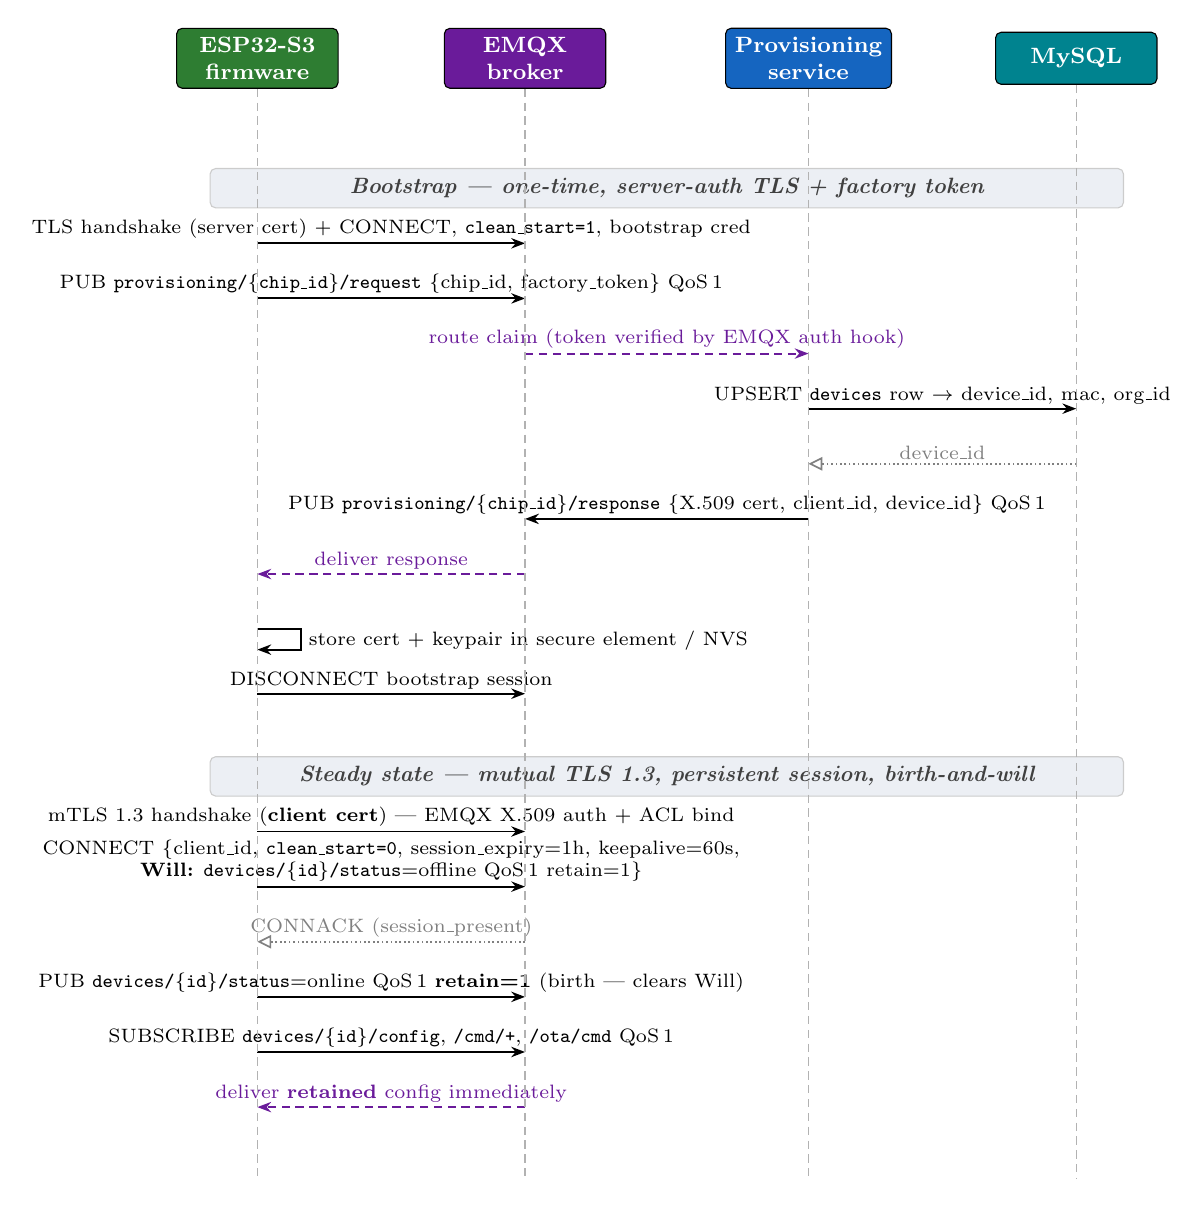
\begin{tikzpicture}
  \def\D{0}\def\B{3.4}\def\P{7.0}\def\M{10.4}
  \def\xmid{5.2}\def\bandw{11.6cm}
  \seqreset
  % headers
  \node[head, fill=devCol] (p0) at (\D,0) {ESP32-S3\\firmware};
  \node[head, fill=brkCol] (p1) at (\B,0) {EMQX\\broker};
  \node[head, fill=svcCol] (p2) at (\P,0) {Provisioning\\service};
  \node[head, fill=dbCol]  (p3) at (\M,0) {MySQL};

  \phase{Bootstrap — one-time, server-auth TLS + factory token}
  \mO{\D}{\B}{TLS handshake (server cert) + CONNECT, \texttt{clean\_start=1}, bootstrap cred}
  \mO{\D}{\B}{PUB \texttt{provisioning/\{chip\_id\}/request} \{chip\_id, factory\_token\} QoS\,1}
  \mA{\B}{\P}{route claim (token verified by EMQX auth hook)}
  \mO{\P}{\M}{UPSERT \texttt{devices} row $\rightarrow$ device\_id, mac, org\_id}
  \mR{\M}{\P}{device\_id}
  \mO{\P}{\B}{PUB \texttt{provisioning/\{chip\_id\}/response} \{X.509 cert, client\_id, device\_id\} QoS\,1}
  \mA{\B}{\D}{deliver response}
  \mS{\D}{store cert + keypair in secure element / NVS}
  \mO{\D}{\B}{DISCONNECT bootstrap session}

  \phase{Steady state — mutual TLS 1.3, persistent session, birth-and-will}
  \mO{\D}{\B}{mTLS 1.3 handshake (\textbf{client cert}) — EMQX X.509 auth + ACL bind}
  \mO{\D}{\B}{CONNECT \{client\_id, \texttt{clean\_start=0}, session\_expiry=1h, keepalive=60s,\\ \textbf{Will:} \texttt{devices/\{id\}/status}=offline QoS\,1 retain=1\}}
  \mR{\B}{\D}{CONNACK (session\_present)}
  \mO{\D}{\B}{PUB \texttt{devices/\{id\}/status}=online QoS\,1 \textbf{retain=1} (birth — clears Will)}
  \mO{\D}{\B}{SUBSCRIBE \texttt{devices/\{id\}/config}, \texttt{/cmd/+}, \texttt{/ota/cmd} QoS\,1}
  \mA{\B}{\D}{deliver \textbf{retained} config immediately}

  % lifelines
  \pgfmathsetmacro{\YBOT}{\YY-0.2}
  \foreach \p in {p0,p1,p2,p3}{\draw[lifeline] (\p.south) -- (\p.south|-0,\YBOT);}
\end{tikzpicture}}
\caption{Phase A — provisioning rotates a factory token into a per-device certificate, then
the production session is established with mutual TLS, a persistent MQTT~5.0 session, and a
retained will/birth pair so presence is never stale.}
\end{figure}

% =====================================================================
\newpage
\section*{3\quad Phase B — Steady-state telemetry (corrected ingestion)}

\begin{figure}[H]
\centering
\resizebox{\textwidth}{!}{%
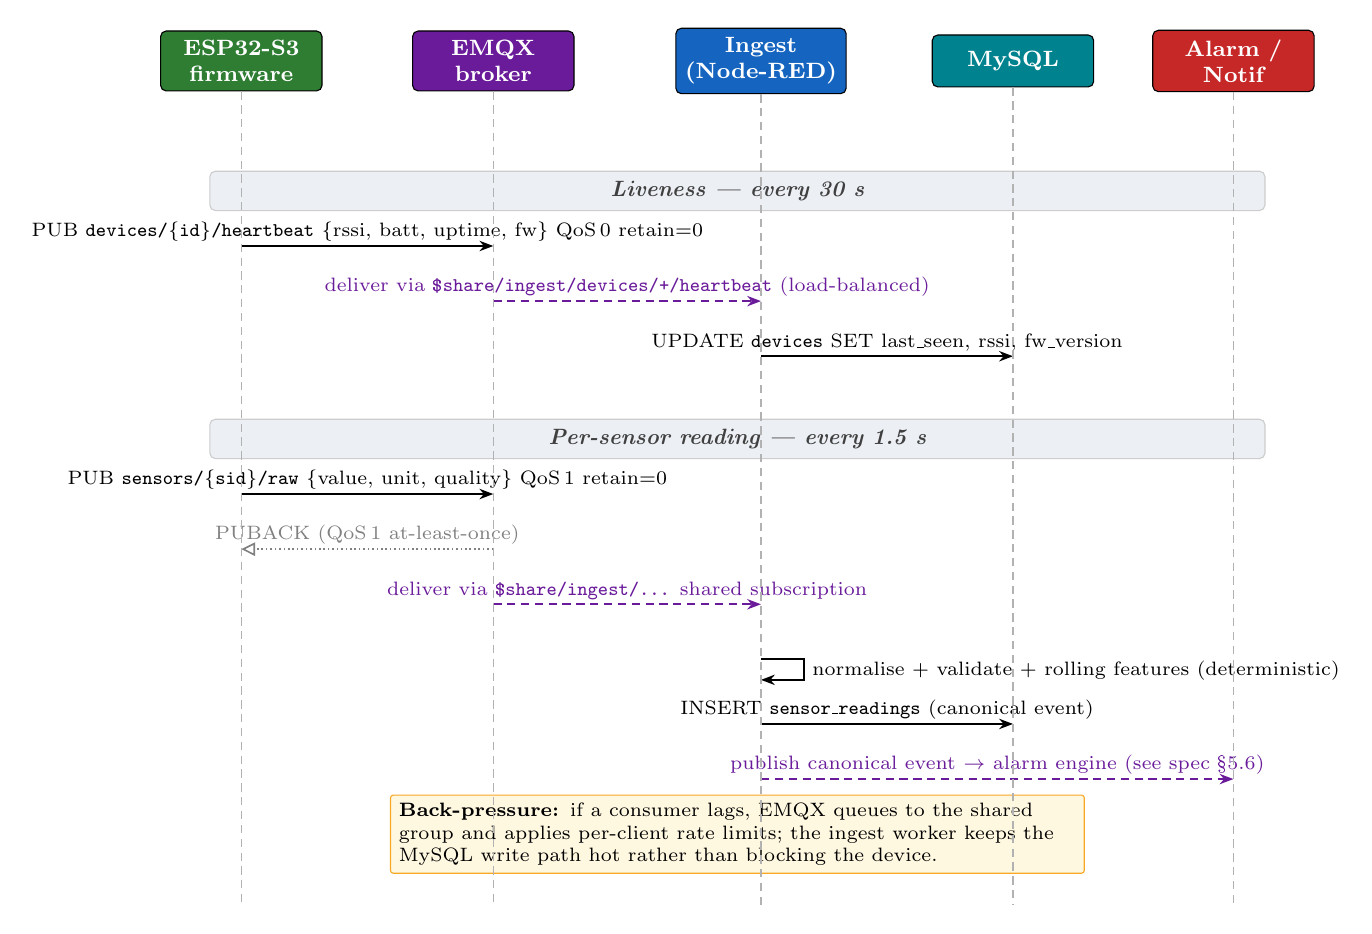
\begin{tikzpicture}
  \def\D{0}\def\B{3.2}\def\I{6.6}\def\M{9.8}\def\A{12.6}
  \def\xmid{6.3}\def\bandw{13.4cm}
  \seqreset
  \node[head, fill=devCol] (p0) at (\D,0) {ESP32-S3\\firmware};
  \node[head, fill=brkCol] (p1) at (\B,0) {EMQX\\broker};
  \node[head, fill=svcCol] (p2) at (\I,0) {Ingest\\(Node-RED)};
  \node[head, fill=dbCol]  (p3) at (\M,0) {MySQL};
  \node[head, fill=usrCol] (p4) at (\A,0) {Alarm /\\Notif};

  \phase{Liveness — every 30 s}
  \mO{\D}{\B}{PUB \texttt{devices/\{id\}/heartbeat} \{rssi, batt, uptime, fw\} QoS\,0 retain=0}
  \mA{\B}{\I}{deliver via \texttt{\$share/ingest/devices/+/heartbeat} (load-balanced)}
  \mO{\I}{\M}{UPDATE \texttt{devices} SET last\_seen, rssi, fw\_version}

  \phase{Per-sensor reading — every 1.5 s}
  \mO{\D}{\B}{PUB \texttt{sensors/\{sid\}/raw} \{value, unit, quality\} QoS\,1 retain=0}
  \mR{\B}{\D}{PUBACK (QoS\,1 at-least-once)}
  \mA{\B}{\I}{deliver via \texttt{\$share/ingest/\dots} shared subscription}
  \mS{\I}{normalise + validate + rolling features (deterministic)}
  \mO{\I}{\M}{INSERT \texttt{sensor\_readings} (canonical event)}
  \mA{\I}{\A}{publish canonical event $\rightarrow$ alarm engine (see spec \S5.6)}

  \note{6.3}{8.6cm}{\textbf{Back-pressure:} if a consumer lags, EMQX queues to the shared
  group and applies per-client rate limits; the ingest worker keeps the MySQL write path
  hot rather than blocking the device.}

  \pgfmathsetmacro{\YBOT}{\YY-0.2}
  \foreach \p in {p0,p1,p2,p3,p4}{\draw[lifeline] (\p.south) -- (\p.south|-0,\YBOT);}
\end{tikzpicture}}
\caption{Phase B — heartbeats stay QoS~0; sensor readings stay QoS~1 with PUBACK. The single
correction that matters for scale is consuming through an EMQX \emph{shared subscription},
which load-balances across ingest replicas and gives the broker a place to absorb back-pressure.}
\end{figure}

% =====================================================================
\newpage
\section*{4\quad Phase C — Signed OTA update with A/B rollback}

\begin{figure}[H]
\centering
\resizebox{\textwidth}{!}{%
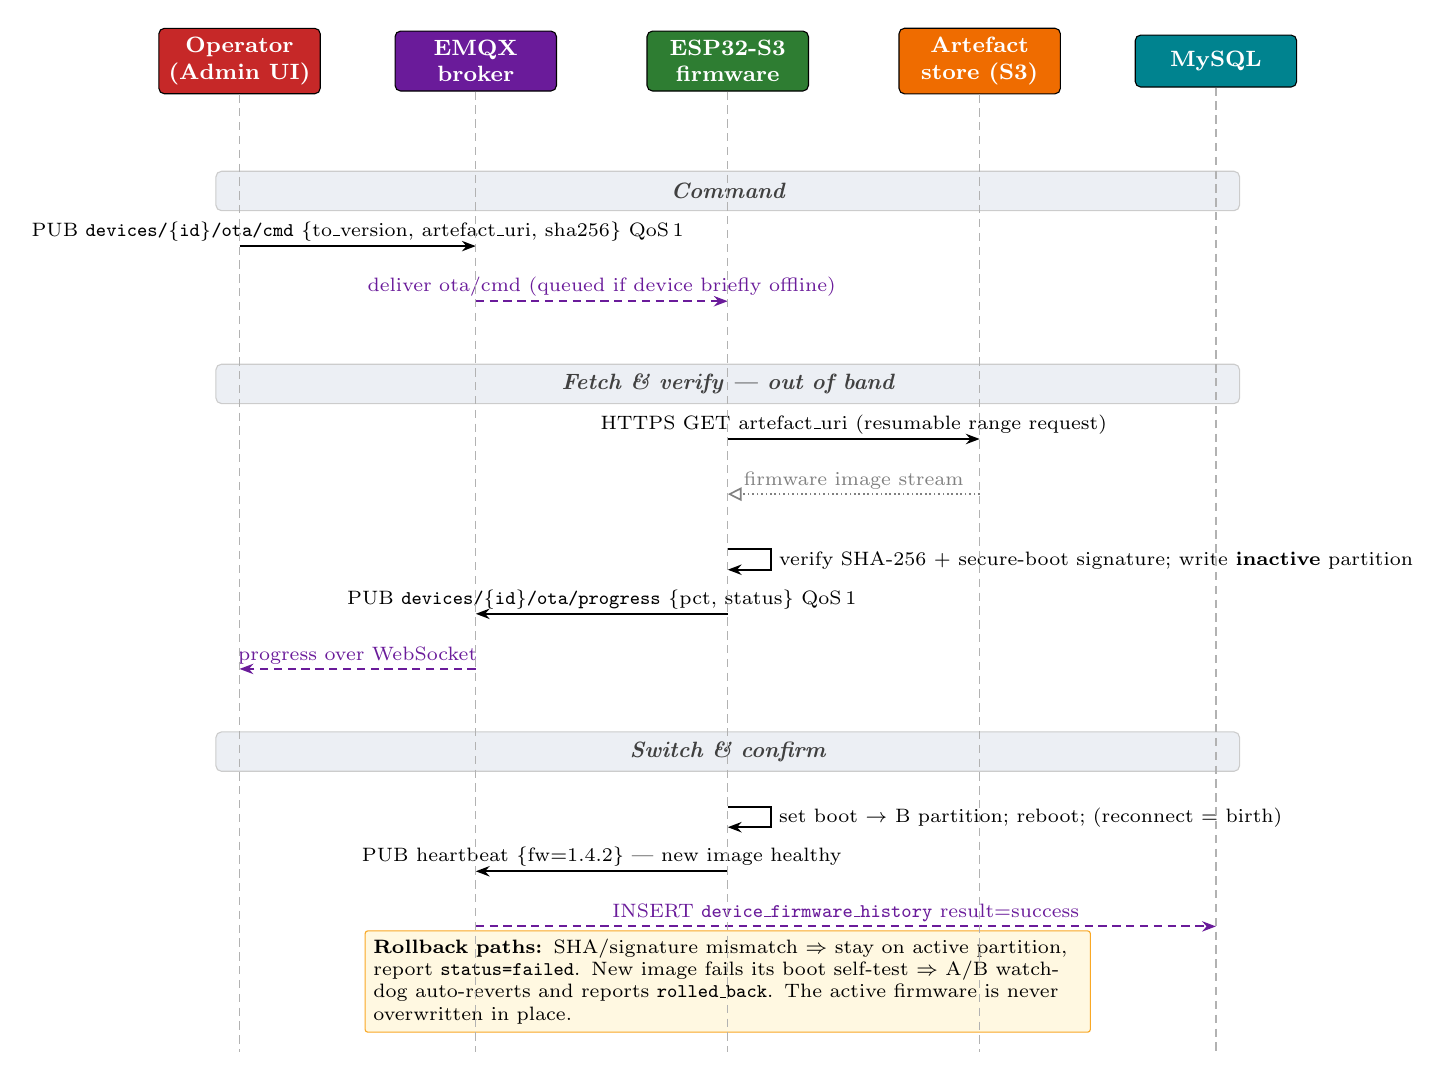
\begin{tikzpicture}
  \def\U{0}\def\B{3.0}\def\D{6.2}\def\O{9.4}\def\M{12.4}
  \def\xmid{6.2}\def\bandw{13.0cm}
  \seqreset
  \node[head, fill=usrCol] (p0) at (\U,0) {Operator\\(Admin UI)};
  \node[head, fill=brkCol] (p1) at (\B,0) {EMQX\\broker};
  \node[head, fill=devCol] (p2) at (\D,0) {ESP32-S3\\firmware};
  \node[head, fill=otaCol] (p3) at (\O,0) {Artefact\\store (S3)};
  \node[head, fill=dbCol]  (p4) at (\M,0) {MySQL};

  \phase{Command}
  \mO{\U}{\B}{PUB \texttt{devices/\{id\}/ota/cmd} \{to\_version, artefact\_uri, sha256\} QoS\,1}
  \mA{\B}{\D}{deliver ota/cmd (queued if device briefly offline)}

  \phase{Fetch \& verify — out of band}
  \mO{\D}{\O}{HTTPS GET artefact\_uri (resumable range request)}
  \mR{\O}{\D}{firmware image stream}
  \mS{\D}{verify SHA-256 + secure-boot signature; write \textbf{inactive} partition}
  \mO{\D}{\B}{PUB \texttt{devices/\{id\}/ota/progress} \{pct, status\} QoS\,1}
  \mA{\B}{\U}{progress over WebSocket}

  \phase{Switch \& confirm}
  \mS{\D}{set boot $\rightarrow$ B partition; reboot; (reconnect = birth)}
  \mO{\D}{\B}{PUB heartbeat \{fw=1.4.2\} — new image healthy}
  \mA{\B}{\M}{INSERT \texttt{device\_firmware\_history} result=success}

  \note{6.2}{9.0cm}{\textbf{Rollback paths:} SHA/signature mismatch $\Rightarrow$ stay on
  active partition, report \texttt{status=failed}. New image fails its boot self-test
  $\Rightarrow$ A/B watchdog auto-reverts and reports \texttt{rolled\_back}. The active
  firmware is never overwritten in place.}

  \pgfmathsetmacro{\YBOT}{\YY-0.2}
  \foreach \p in {p0,p1,p2,p3,p4}{\draw[lifeline] (\p.south) -- (\p.south|-0,\YBOT);}
\end{tikzpicture}}
\caption{Phase C — OTA is delivered as a signed artefact fetched out of band over HTTPS,
flashed to the inactive A/B slot, and only promoted after verification; the firmware
version reported in the next heartbeat closes the audit loop.}
\end{figure}

% =====================================================================
\section*{5\quad Phase D — Ungraceful disconnect (Last Will \& Testament)}

\begin{figure}[H]
\centering
\resizebox{0.92\textwidth}{!}{%
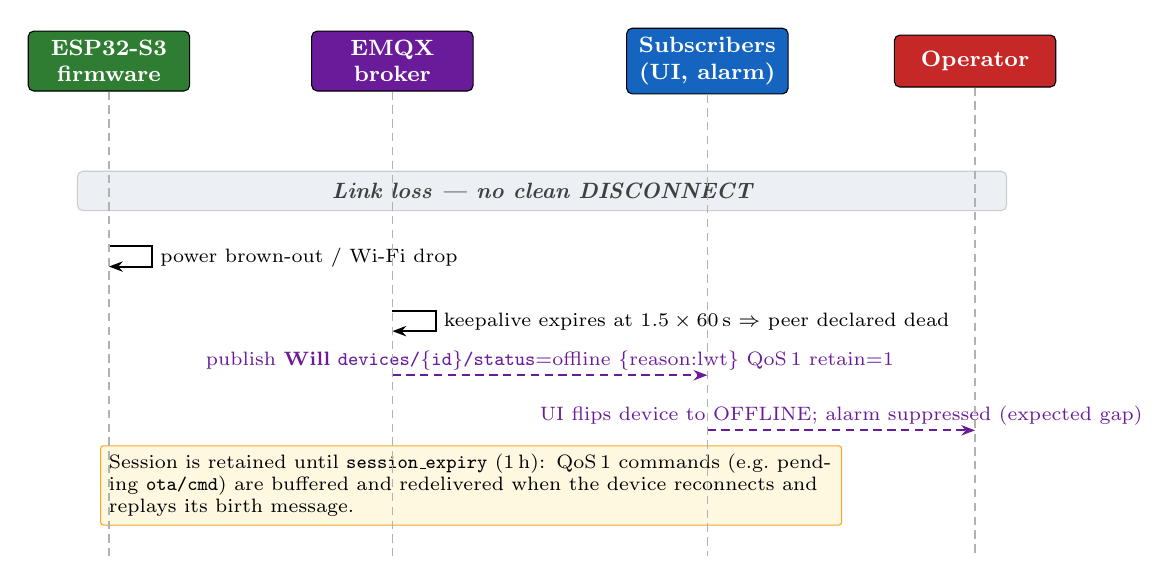
\begin{tikzpicture}
  \def\D{0}\def\B{3.6}\def\S{7.6}\def\U{11.0}
  \def\xmid{5.5}\def\bandw{11.8cm}
  \seqreset
  \node[head, fill=devCol] (p0) at (\D,0) {ESP32-S3\\firmware};
  \node[head, fill=brkCol] (p1) at (\B,0) {EMQX\\broker};
  \node[head, fill=svcCol] (p2) at (\S,0) {Subscribers\\(UI, alarm)};
  \node[head, fill=usrCol] (p3) at (\U,0) {Operator};

  \phase{Link loss — no clean DISCONNECT}
  \mS{\D}{power brown-out / Wi-Fi drop}
  \mS{\B}{keepalive expires at $1.5\times60$\,s $\Rightarrow$ peer declared dead}
  \mA{\B}{\S}{publish \textbf{Will} \texttt{devices/\{id\}/status}=offline \{reason:lwt\} QoS\,1 retain=1}
  \mA{\S}{\U}{UI flips device to OFFLINE; alarm suppressed (expected gap)}
  \note{4.6}{9.2cm}{Session is retained until \texttt{session\_expiry} (1\,h): QoS\,1 commands
  (e.g.\ pending \texttt{ota/cmd}) are buffered and redelivered when the device reconnects
  and replays its birth message.}

  \pgfmathsetmacro{\YBOT}{\YY-0.2}
  \foreach \p in {p0,p1,p2,p3}{\draw[lifeline] (\p.south) -- (\p.south|-0,\YBOT);}
\end{tikzpicture}}
\caption{Phase D — because the Will is registered at CONNECT with retain=1, presence stays
correct without any device cooperation; the retained session keeps queued commands alive
across the outage.}
\end{figure}

% =====================================================================
\newpage
\section*{6\quad Per-product telemetry — one envelope, three payload profiles}
The phases above are deliberately product-agnostic because every device speaks the
\emph{same} firmware contract. Temperature is transmitted by all three product lines, but it
is only \emph{one channel} inside a product-specific set. A device emits \textbf{one
\texttt{sensors/\{sid\}/raw} publish per channel per cycle}; the broker and ingest path are
identical, and the meaning of each \texttt{sensor\_id} is resolved by the polymorphic
\emph{CTI} model (\texttt{sensors.host\_fk} $\in\{$t,c,b$\}$ $\to$ exactly one of the three
\texttt{*\_sensor\_specs} tables). What actually differs per product is the
\emph{channel set}, units, and cadence.

\begin{center}
\renewcommand{\arraystretch}{1.3}
\small
\begin{tabularx}{\textwidth}{@{}p{3.5cm} c X@{}}
\toprule
\textbf{Product line (host)} & \textbf{Cadence} & \textbf{Channels emitted as \texttt{sensors/\{sid\}/raw}} \\
\midrule
\textbf{Refrigeration} \newline Data Logger \newline (\texttt{carbonbox}, host=\texttt{c}) &
  temp 30--60\,s; \newline door on-change &
  \texttt{temp\_c} ($^\circ$C); \texttt{door\_state} (bool 0/1 — \emph{event}, not a scalar
  measurement). Cold-chain min/max only. \\
\addlinespace[2pt]
\textbf{BloodBOX} \newline (host=\texttt{b}) &
  temp/RH 10--30\,s; \newline GPS 1--5\,s in transit; \newline impact event-driven &
  \texttt{temp\_c}, \texttt{rh\_pct} (humidity), \texttt{batt\_pct}, \texttt{impact\_g}
  (shock), \texttt{gps} (lat/lng — \emph{compound}), \texttt{baro\_alt\_m} (floor/altitude).
  Medical transit; richest payload. \\
\addlinespace[2pt]
\textbf{Transformer} \newline Monitoring \newline (\texttt{eternity}, host=\texttt{t}) &
  thermal 30--60\,s; \newline DGA minutes--hours &
  \texttt{oil\_temp\_c}, \texttt{ambient\_temp\_c}, \texttt{dga\_h2\_ppm} (dissolved
  hydrogen), \texttt{moisture\_pct}, \texttt{oil\_level\_pct}, \texttt{load\_pct}.
  Multi-channel DGA + thermal. \\
\bottomrule
\end{tabularx}
\end{center}

\noindent\textbf{The deltas the generic envelope must absorb:} \texttt{door\_state} and
\texttt{impact\_g} are boolean/event channels mapped as \texttt{value}$\in\{0,1\}$ /
\texttt{unit=event}; \texttt{gps} is a compound channel (sent as two readings \texttt{lat},
\texttt{lng} or one structured value); cadences span three orders of magnitude (GPS seconds
vs.\ DGA hours). None of this changes the topic or QoS — only the channel set and the spec
table the ingest worker joins to.

\begin{figure}[H]
\centering
\resizebox{\textwidth}{!}{%
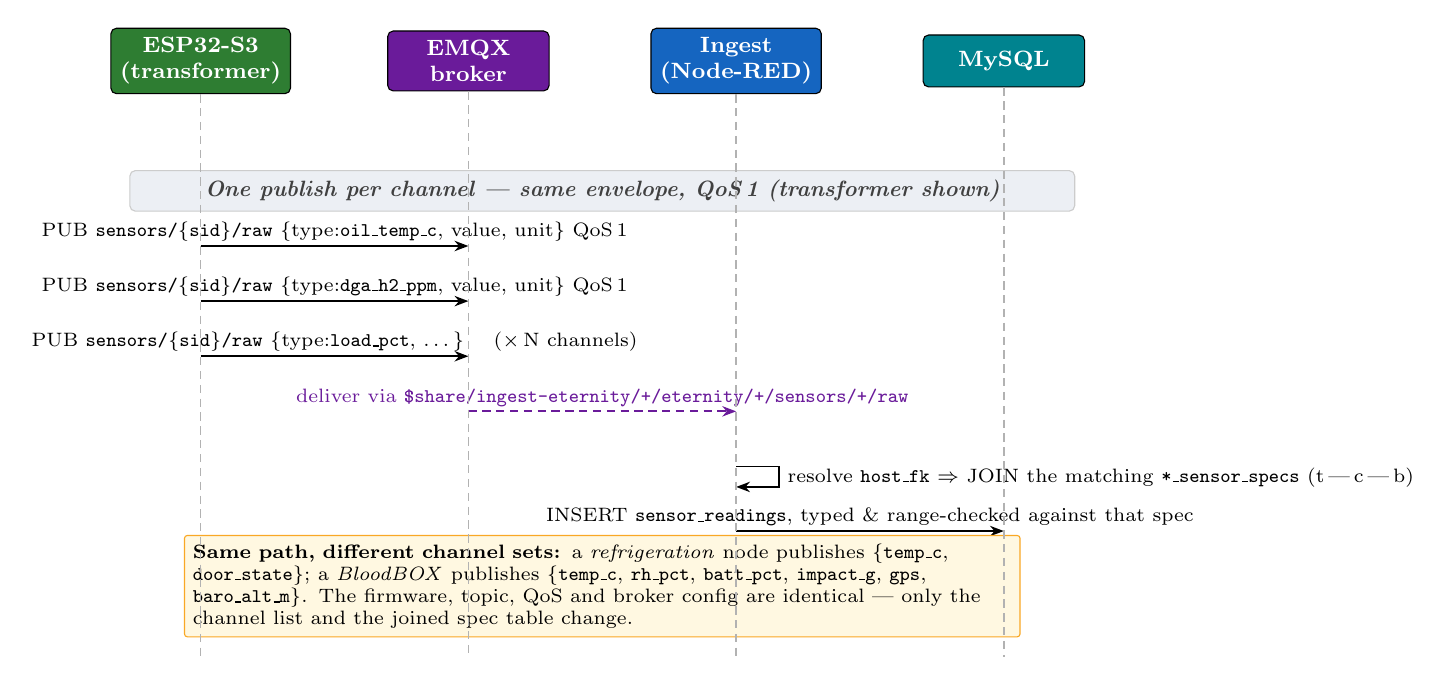
\begin{tikzpicture}
  \def\D{0}\def\B{3.4}\def\I{6.8}\def\M{10.2}
  \def\xmid{5.1}\def\bandw{12.0cm}
  \seqreset
  \node[head, fill=devCol] (p0) at (\D,0) {ESP32-S3\\(transformer)};
  \node[head, fill=brkCol] (p1) at (\B,0) {EMQX\\broker};
  \node[head, fill=svcCol] (p2) at (\I,0) {Ingest\\(Node-RED)};
  \node[head, fill=dbCol]  (p3) at (\M,0) {MySQL};

  \phase{One publish per channel — same envelope, QoS\,1 (transformer shown)}
  \mO{\D}{\B}{PUB \texttt{sensors/\{sid\}/raw} \{type:\texttt{oil\_temp\_c}, value, unit\} QoS\,1}
  \mO{\D}{\B}{PUB \texttt{sensors/\{sid\}/raw} \{type:\texttt{dga\_h2\_ppm}, value, unit\} QoS\,1}
  \mO{\D}{\B}{PUB \texttt{sensors/\{sid\}/raw} \{type:\texttt{load\_pct}, \dots\} \quad($\times$\,N channels)}
  \mA{\B}{\I}{deliver via \texttt{\$share/ingest-eternity/+/eternity/+/sensors/+/raw}}
  \mS{\I}{resolve \texttt{host\_fk} $\Rightarrow$ JOIN the matching \texttt{*\_sensor\_specs} (t\,|\,c\,|\,b)}
  \mO{\I}{\M}{INSERT \texttt{sensor\_readings}, typed \& range-checked against that spec}

  \note{5.1}{10.4cm}{\textbf{Same path, different channel sets:} a \emph{refrigeration} node
  publishes \{\texttt{temp\_c}, \texttt{door\_state}\}; a \emph{BloodBOX} publishes
  \{\texttt{temp\_c}, \texttt{rh\_pct}, \texttt{batt\_pct}, \texttt{impact\_g}, \texttt{gps},
  \texttt{baro\_alt\_m}\}. The firmware, topic, QoS and broker config are identical — only the
  channel list and the joined spec table change.}

  \pgfmathsetmacro{\YBOT}{\YY-0.2}
  \foreach \p in {p0,p1,p2,p3}{\draw[lifeline] (\p.south) -- (\p.south|-0,\YBOT);}
\end{tikzpicture}}
\caption{Phase B (per-product) — each device fans out one reading per channel over the single
\texttt{sensors/\{sid\}/raw} envelope; the ingest worker resolves the polymorphic host FK and
joins the correct per-type spec table, so a 6-channel transformer and a 2-channel fridge share
one pipeline.}
\end{figure}

% =====================================================================
\newpage
\section*{7\quad Per-product topic namespace (corrected)}
Phases A--D used the device-rooted \emph{tail} of each topic (\texttt{devices/\{id\}/\dots},
\texttt{sensors/\{sid\}/\dots}) for legibility. The complete, ACL-enforceable form prefixes
\textbf{every} production topic with
\texttt{\{tenant\}/\allowbreak\{product\}/\allowbreak\{device\_id\}}, where
\texttt{product} $\in\{$\texttt{eternity}, \texttt{carbonbox}, \texttt{bloodbox}$\}$. The
prefix is not cosmetic — it is what lets one broker host three products without cross-talk.

\paragraph{Why product belongs in the topic (EMQX best practice).}
\begin{itemize}[leftmargin=1.4em,itemsep=1pt]
  \item \textbf{Isolation \& ACL:} the cert CN is \texttt{\{tenant\}.\{product\}.\{device\}};
        EMQX templates one allow rule \texttt{\$\{cn\_tenant\}/\$\{cn\_product\}/\$\{cn\_device\}/\#}
        and denies everything else. A device physically cannot publish into another product.
  \item \textbf{Per-product ingest pools:} each product runs its own shared-subscription group
        (\texttt{\$share/\allowbreak ingest-eternity/\dots}), because the processing differs — DGA gas-trend
        models, fridge door-debounce, BloodBOX GPS + excursion timers.
  \item \textbf{Per-product schema, retention, alarm thresholds} (\S8) are keyed off the
        \texttt{product} segment with no payload sniffing.
  \item \textbf{Fleet analytics by wildcard:} \texttt{+/eternity/\#} = every transformer across
        all tenants (superadmin); \texttt{acme/\#} = one tenant, all products.
\end{itemize}

\begin{center}
\renewcommand{\arraystretch}{1.22}
\small
\begin{tabularx}{\textwidth}{@{}l c c c X@{}}
\toprule
\textbf{Topic} & \textbf{Dir} & \textbf{QoS} & \textbf{Ret} & \textbf{Notes} \\
\midrule
\multicolumn{5}{@{}l}{\itshape Bootstrap listener — pre-identity, flat namespace}\\
\texttt{provisioning/\{chip\_id\}/request}  & D$\to$B & 1 & 0 & claim with factory token \\
\texttt{provisioning/\{chip\_id\}/response} & B$\to$D & 1 & 0 & returns X.509 cert + client\_id \\
\addlinespace[2pt]
\multicolumn{5}{@{}l}{\itshape Production listener — prefix \texttt{P\,=\,\{tenant\}/\{product\}/\{device\_id\}}}\\
\texttt{P/status}              & D$\to$B & 1 & \textbf{1} & Will \emph{and} birth \\
\texttt{P/heartbeat}           & D$\to$B & 0 & 0 & 30\,s; liveness \& fw\_version \\
\texttt{P/sensors/\{sid\}/raw} & D$\to$B & 1 & 0 & per-channel reading; ingest via \texttt{\$share} \\
\texttt{P/alarm/\{sid\}}       & B$\to\star$ & 1 & \textbf{1} & alarm-engine state, retained (\S9) \\
\texttt{P/config}              & B$\to$D & 1 & \textbf{1} & retained; \textbf{per-product thresholds} (\S8) \\
\texttt{P/cmd/\{op\}}          & B$\to$D & 1 & 0 & reboot / calibrate / set-threshold \\
\texttt{P/ota/cmd}             & B$\to$D & 1 & 0 & signed artefact descriptor \\
\texttt{P/ota/progress}        & D$\to$B & 1 & 0 & percent + status \\
\bottomrule
\end{tabularx}
\\[3pt]
{\footnotesize $\star$ = subscribers: UI (WebSocket bridge), notification service, and
optionally the device itself for actuation.}
\end{center}

\paragraph{Per-product shared subscriptions \& ACL roles.}
\begin{center}
\small
\begin{tabularx}{\textwidth}{@{}l X@{}}
\toprule
\textbf{Role} & \textbf{Authorised topic filter} \\
\midrule
device (each) & pub+sub \texttt{\{tenant\}/\{product\}/\{device\}/\#} only \\
ingest-eternity   & sub \texttt{\$share/ingest-eternity/+/eternity/+/sensors/+/raw} \\
ingest-carbonbox  & sub \texttt{\$share/ingest-carbonbox/+/carbonbox/+/sensors/+/raw} \\
ingest-bloodbox   & sub \texttt{\$share/ingest-bloodbox/+/bloodbox/+/sensors/+/raw} \\
alarm-engine & pub \texttt{+/+/+/alarm/+}; \quad sub \texttt{+/+/+/sensors/+/raw} \\
ui / notif   & sub \texttt{\{tenant\}/\#} (tenant-scoped, read-only) \\
\bottomrule
\end{tabularx}
\end{center}

% =====================================================================
\newpage
\section*{8\quad Per-product alarm thresholds}
Thresholds are \textbf{not} compiled into firmware. They ship in the retained
\texttt{P/config} payload (\S7), so the alarm engine and the device's edge fast-path share one
source of truth and an operator can retune without an OTA. The values below are taken from the
current product logic in \texttt{src/lib/}; rows marked \emph{(proposed)} have no hardcoded
value yet and are filled with defensible medical/industrial defaults.

\begin{center}
\renewcommand{\arraystretch}{1.18}
\small
\begin{tabularx}{\textwidth}{@{}l c r r c X@{}}
\toprule
\textbf{Channel} & \textbf{Unit} & \textbf{Warn} & \textbf{Crit} & \textbf{Dir} & \textbf{Guard / debounce} \\
\midrule
\multicolumn{6}{@{}l}{\textbf{Transformer — \texttt{eternity} (host\,=\,t)}}\\
\texttt{oil\_temp\_c}     & $^\circ$C & 80  & 95   & $\uparrow$ & WARN after 2 consecutive readings \\
\texttt{ambient\_temp\_c} & $^\circ$C & 40  & 50   & $\uparrow$ & \\
\texttt{dga\_h2\_ppm}     & ppm & 150 & 300  & $\uparrow$ & slow DGA cadence; trend-aware \\
\texttt{moisture\_ppm}    & ppm & 25  & 35   & $\uparrow$ & \\
\texttt{oil\_level\_pct}  & \% & 70  & 60   & $\downarrow$ & \textbf{inverted} (low = bad) \\
\texttt{load\_pct}        & \% & 80  & 95   & $\uparrow$ & \\
\addlinespace[2pt]
\multicolumn{6}{@{}l}{\textbf{Refrigeration — \texttt{carbonbox} (host\,=\,c)}}\\
\texttt{temp\_c}     & $^\circ$C & 6 & 8 & $\uparrow$ & WARN $>$6 after 2 readings \\
\texttt{door\_state} & bool & --- & open & --- & CRITICAL; corrected: debounce $>$60\,s \\
\texttt{online}      & bool & --- & offline & --- & CRITICAL after $1.5\times$HB ($\approx$90\,s) \\
\addlinespace[2pt]
\multicolumn{6}{@{}l}{\textbf{BloodBOX — \texttt{bloodbox} (host\,=\,b)}}\\
\texttt{temp\_c}    & $^\circ$C & 6 & 7 & $\uparrow$ & medical: no debounce \\
\texttt{excursion}  & $^\circ$C & --- & $>$\,maxTempC (8) & $\uparrow$ & \textbf{per-transit} limit + excursion-time audit \\
\texttt{rh\_pct}    & \% & 80 & 90 & $\uparrow$ & humidity \emph{(proposed)} \\
\texttt{batt\_pct}  & \% & 40 & 20 & $\downarrow$ & low = bad \\
\texttt{impact\_g}  & g  & --- & 3.0 & $\uparrow$ & single-sample event $\Rightarrow$ CRITICAL \\
\texttt{lid\_state} & bool & open & --- & --- & WARNING on open \\
\bottomrule
\end{tabularx}
\end{center}
\noindent{\footnotesize Direction: $\uparrow$ = high value is bad, $\downarrow$ = low value is
bad. \texttt{door\_state}/\texttt{impact\_g}/\texttt{lid\_state} are event channels (\S6).}

\paragraph{Retained \texttt{P/config} threshold payloads (one per product).}
\small
\begin{verbatim}
eternity:  {"product":"eternity","sample_s":30,"dga_sample_s":3600,
  "thresholds":{
    "oil_temp_c":   {"warn":80,"crit":95,"dir":"high","debounce_n":2},
    "ambient_temp_c":{"warn":40,"crit":50,"dir":"high","debounce_n":2},
    "dga_h2_ppm":   {"warn":150,"crit":300,"dir":"high"},
    "moisture_ppm": {"warn":25,"crit":35,"dir":"high"},
    "oil_level_pct":{"warn":70,"crit":60,"dir":"low"},
    "load_pct":     {"warn":80,"crit":95,"dir":"high"}}}

carbonbox: {"product":"carbonbox","sample_s":30,
  "thresholds":{
    "temp_c":     {"warn":6,"crit":8,"dir":"high","debounce_n":2},
    "door_state": {"crit_after_s":60},
    "online":     {"crit_after_s":90}}}

bloodbox:  {"product":"bloodbox","sample_s":15,"gps_sample_s":3,
  "thresholds":{
    "temp_c":    {"warn":6,"crit":7,"dir":"high"},
    "excursion": {"max_temp_c":8,"audit":true},
    "rh_pct":    {"warn":80,"crit":90,"dir":"high"},
    "batt_pct":  {"warn":40,"crit":20,"dir":"low"},
    "impact_g":  {"crit":3.0,"event":true},
    "lid_state": {"warn_on_open":true}}}
\end{verbatim}
\normalsize

% =====================================================================
\newpage
\section*{9\quad Alarm semantics \& state machine per product}
The alarm engine is the canonical owner of state; the device never decides an alarm row (it may
only raise an \emph{edge} hint). State follows the spec \S5.5 lifecycle, with these
per-product guard differences:
\begin{center}
NORMAL $\to$ WARNING $\to$ CRITICAL $\to$ ACKNOWLEDGED $\to$ ESCALATED $\to$ CLEARED
\end{center}

\begin{center}
\renewcommand{\arraystretch}{1.28}
\small
\begin{tabularx}{\textwidth}{@{}p{2.6cm} X@{}}
\toprule
\textbf{Product} & \textbf{Guard differences vs.\ the shared \S5.5 lifecycle} \\
\midrule
\textbf{eternity} & WARNING requires 2 consecutive over-threshold readings; CRITICAL is
  immediate at $\geq$crit. \texttt{oil\_level} inverted. One alarm \emph{row per channel}; DGA
  evaluated on a slow cadence with a rising-trend pre-empt. \\
\textbf{carbonbox} & \texttt{door\_state}=open and \texttt{online}=offline \textbf{bypass} the
  2-reading debounce $\Rightarrow$ immediate CRITICAL (safety). The corrected design adds a
  60\,s door debounce so routine access does not nuisance-trip. \\
\textbf{bloodbox} & Temperature is medical $\Rightarrow$ no debounce. The CRITICAL bound is the
  \textbf{per-transit} \texttt{maxTempC} (mobile, default 8), tracked with an excursion-time
  audit trail. \texttt{impact\_g} is a single-sample event; \texttt{batt\_pct} low. \\
\bottomrule
\end{tabularx}
\end{center}

\begin{figure}[H]
\centering
\resizebox{\textwidth}{!}{%
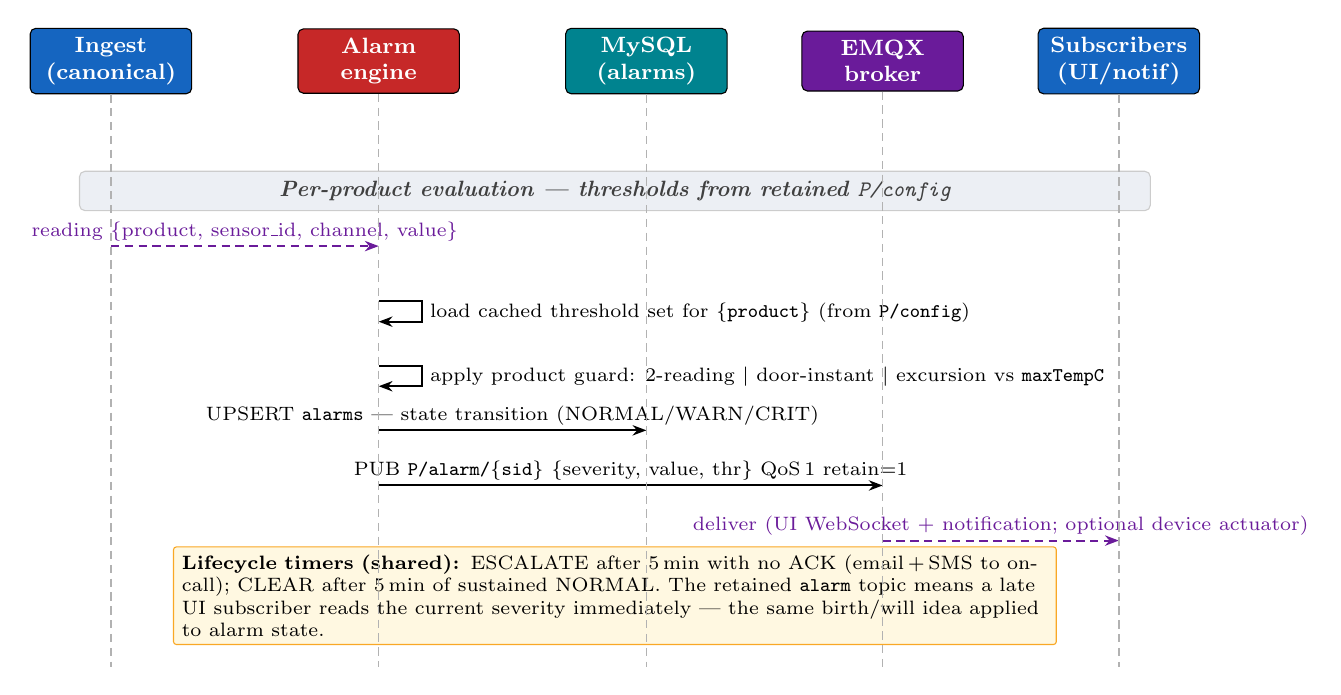
\begin{tikzpicture}
  \def\I{0}\def\E{3.4}\def\M{6.8}\def\B{9.8}\def\S{12.8}
  \def\xmid{6.4}\def\bandw{13.6cm}
  \seqreset
  \node[head, fill=svcCol] (p0) at (\I,0) {Ingest\\(canonical)};
  \node[head, fill=usrCol] (p1) at (\E,0) {Alarm\\engine};
  \node[head, fill=dbCol]  (p2) at (\M,0) {MySQL\\(alarms)};
  \node[head, fill=brkCol] (p3) at (\B,0) {EMQX\\broker};
  \node[head, fill=svcCol] (p4) at (\S,0) {Subscribers\\(UI/notif)};

  \phase{Per-product evaluation — thresholds from retained \texttt{P/config}}
  \mA{\I}{\E}{reading \{product, sensor\_id, channel, value\}}
  \mS{\E}{load cached threshold set for \texttt{\{product\}} (from \texttt{P/config})}
  \mS{\E}{apply product guard: 2-reading $|$ door-instant $|$ excursion vs \texttt{maxTempC}}
  \mO{\E}{\M}{UPSERT \texttt{alarms} — state transition (NORMAL/WARN/CRIT)}
  \mO{\E}{\B}{PUB \texttt{P/alarm/\{sid\}} \{severity, value, thr\} QoS\,1 retain=1}
  \mA{\B}{\S}{deliver (UI WebSocket + notification; optional device actuator)}

  \note{6.4}{11.0cm}{\textbf{Lifecycle timers (shared):} ESCALATE after 5\,min with no ACK
  (email\,+\,SMS to on-call); CLEAR after 5\,min of sustained NORMAL. The retained
  \texttt{alarm} topic means a late UI subscriber reads the current severity immediately —
  the same birth/will idea applied to alarm state.}

  \pgfmathsetmacro{\YBOT}{\YY-0.2}
  \foreach \p in {p0,p1,p2,p3,p4}{\draw[lifeline] (\p.south) -- (\p.south|-0,\YBOT);}
\end{tikzpicture}}
\caption{Phase E — one alarm engine, three threshold sets. The reading carries its
\texttt{product}; the engine loads that product's thresholds and guard, transitions the
\texttt{alarms} row per \S5.5, and republishes the result on the retained per-device
\texttt{alarm} topic so presence-of-alarm is never stale.}
\end{figure}

\paragraph{EMQX configuration checklist.}
\begin{itemize}[leftmargin=1.4em,itemsep=1pt]
  \item Dedicated TLS listeners: a \emph{bootstrap} listener (server-auth, token) and a
        \emph{production} listener (mutual TLS, \texttt{verify=verify\_peer},
        \texttt{fail\_if\_no\_peer\_cert=true}).
  \item Authentication chain: X.509 CN \texttt{\{tenant\}.\{product\}.\{device\}}
        $\rightarrow$ \texttt{client\_id}; reject mismatched or duplicate client IDs.
  \item Authorization (ACL) templated from the CN so each device is boxed into
        \texttt{\{tenant\}/\allowbreak\{product\}/\allowbreak\{device\}/\#} (\S7).
  \item One shared-subscription group \emph{per product} for ingest; alarm engine and UI on
        their own scoped roles; never a single static subscriber.
  \item Flapping detection + per-client rate \& bandwidth limits enabled.
  \item Session expiry sized to the longest tolerable command-delivery gap (here 1\,h).
\end{itemize}

% =====================================================================
%  Part II (Hardware) + Part III (Firmware concept)
%  \input by esp32-platform-spec.tex
% =====================================================================

\part*{Part II\quad Hardware: ESP32-S3 PCB}
\addcontentsline{toc}{part}{Part II — Hardware: ESP32-S3 PCB}

\section*{10\quad PCB function map}
The board is an ESP32-S3-WROOM-1 (N16R8) carrier exposing every field interface the three
products need. One firmware drives all of them; which interfaces are \emph{active} is chosen by
the product profile (\S12).

\paragraph{Functional blocks.}
\begin{itemize}[leftmargin=1.4em,itemsep=1pt]
  \item \textbf{MCU core} — ESP32-S3-WROOM-1 (N16R8): 16\,MB flash, 8\,MB PSRAM, Wi-Fi + BLE;
        decoupling C2 10\,$\mu$F, C10/C4 0.1\,$\mu$F.
  \item \textbf{System / boot} — Reset (\texttt{EN}, R13 10\,k$\Omega$, RST button), Boot/download
        (\texttt{IO0}, R20 10\,k$\Omega$, PROG button), JTAG (\texttt{MTDI/MTDO/MTCK}).
  \item \textbf{Power} — PWR 12\,V in (IN+/IN--), battery B+, rails 12\,V $\to$ 5\,V $\to$ 3.3\,V.
  \item \textbf{Communication} — CAN (SN65HVD230, 120\,$\Omega$ term), RS-485 (MAX3485, 120\,$\Omega$ term),
        4G-UART, LoRa E220-900, USB (native), I\textsuperscript{2}C.
  \item \textbf{Field I/O} — digital inputs (DI), digital outputs (DO1/DO2 @ 12\,V), CT
        (current, ADC), TM1.
  \item \textbf{HMI / storage} — LCD (I\textsuperscript{2}C), SD card, status LEDs (GPIO47 green, GPIO48 red).
  \item \textbf{Timekeeping} — \textbf{external RTC (DS3231}, TCXO $\pm$2\,ppm) on I\textsuperscript{2}C + CR2032 coin
        cell — holds wall-clock across brown-out and offline windows so every SD-buffered sample and
        alarm is auditable (\S10.1).
\end{itemize}

\begin{figure}[H]
\centering
\resizebox{\textwidth}{!}{%
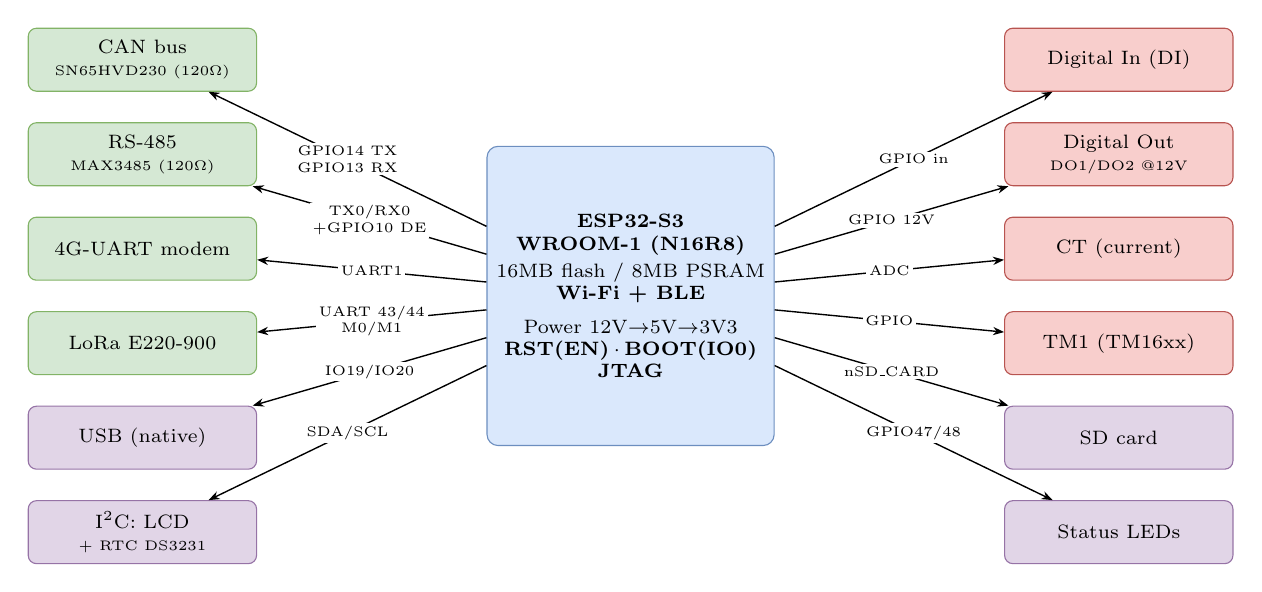
\begin{tikzpicture}[node distance=0pt]
  % centre MCU
  \node[draw=hwEdge, fill=hwCol, rounded corners=4pt, align=center, font=\scriptsize\bfseries,
        minimum width=3.6cm, minimum height=3.8cm] (mcu)
    {ESP32-S3\\WROOM-1 (N16R8)\\[2pt]\normalfont 16MB flash / 8MB PSRAM\\Wi-Fi + BLE\\[4pt]
     \normalfont Power 12V$\to$5V$\to$3V3\\RST(EN)\,$\cdot$\,BOOT(IO0)\\JTAG};
  % left column (communication)
  \def\lx{-6.2}
  \node[periph={drvCol}{drvEdge}] (can)  at (\lx, 3.0){CAN bus\\\tiny SN65HVD230 (120$\Omega$)};
  \node[periph={drvCol}{drvEdge}] (rs)   at (\lx, 1.8){RS-485\\\tiny MAX3485 (120$\Omega$)};
  \node[periph={drvCol}{drvEdge}] (g4)   at (\lx, 0.6){4G-UART modem};
  \node[periph={drvCol}{drvEdge}] (lora) at (\lx,-0.6){LoRa E220-900};
  \node[periph={cloudCol}{cloudEdge}] (usb) at (\lx,-1.8){USB (native)};
  \node[periph={cloudCol}{cloudEdge}] (i2c) at (\lx,-3.0){I\textsuperscript{2}C: LCD\\\tiny + RTC DS3231};
  % right column (field I/O + HMI)
  \def\rx{6.2}
  \node[periph={crossCol}{crossEdge}] (di)  at (\rx, 3.0){Digital In (DI)};
  \node[periph={crossCol}{crossEdge}] (do)  at (\rx, 1.8){Digital Out\\\tiny DO1/DO2 @12V};
  \node[periph={crossCol}{crossEdge}] (ct)  at (\rx, 0.6){CT (current)};
  \node[periph={crossCol}{crossEdge}] (tm1) at (\rx,-0.6){TM1 (TM16xx)};
  \node[periph={cloudCol}{cloudEdge}] (sd)  at (\rx,-1.8){SD card};
  \node[periph={cloudCol}{cloudEdge}] (led) at (\rx,-3.0){Status LEDs};
  % edges with GPIO labels
  \tikzset{e/.style={-{Stealth[length=4pt]}, line width=0.5pt}}
  \draw[e] (mcu) -- (can)  node[elab,midway]{GPIO14 TX\\GPIO13 RX};
  \draw[e] (mcu) -- (rs)   node[elab,midway]{TX0/RX0\\+GPIO10 DE};
  \draw[e] (mcu) -- (g4)   node[elab,midway]{UART1};
  \draw[e] (mcu) -- (lora) node[elab,midway]{UART 43/44\\M0/M1};
  \draw[e] (mcu) -- (usb)  node[elab,midway]{IO19/IO20};
  \draw[e] (mcu) -- (i2c)  node[elab,midway]{SDA/SCL};
  \draw[e] (mcu) -- (di)   node[elab,midway]{GPIO in};
  \draw[e] (mcu) -- (do)   node[elab,midway]{GPIO 12V};
  \draw[e] (mcu) -- (ct)   node[elab,midway]{ADC};
  \draw[e] (mcu) -- (tm1)  node[elab,midway]{GPIO};
  \draw[e] (mcu) -- (sd)   node[elab,midway]{nSD\_CARD};
  \draw[e] (mcu) -- (led)  node[elab,midway]{GPIO47/48};
\end{tikzpicture}}
\caption{ESP32-S3 PCB — function \& signal-flow map (communication left, field-I/O \& HMI right;
edge labels are the GPIO / signal nets).}
\end{figure}

\paragraph{Per-product sensor $\to$ interface.}
\begin{center}
\renewcommand{\arraystretch}{1.2}\small
\begin{tabularx}{\textwidth}{@{}l X@{}}
\toprule
\textbf{Product} & \textbf{Channels (PCB interface)} \\
\midrule
bloodBOX (b) & \texttt{temp\_c}(I\textsuperscript{2}C), \texttt{rh\_pct}(I\textsuperscript{2}C), \texttt{batt\_pct}(ADC),
  \texttt{impact\_g}(I\textsuperscript{2}C accel), \texttt{gps}(UART), \texttt{baro\_alt\_m}(I\textsuperscript{2}C) \\
refrigeDataLogger (c) & \texttt{temp\_c}(I\textsuperscript{2}C/1-wire), \texttt{door\_state}(DI, debounced),
  \texttt{online}(link) \\
transformersMonitoring (t) & \texttt{oil\_temp\_c}(RS485/ADC), \texttt{ambient\_temp\_c}(I\textsuperscript{2}C),
  \texttt{dga\_h2\_ppm}(RS485), \texttt{moisture\_ppm}(RS485), \texttt{oil\_level\_pct}(ADC),
  \texttt{load\_pct}(CT) \\
\bottomrule
\end{tabularx}
\end{center}
{\footnotesize Interface assignments are concept-level intent from the PCB map; confirm against
the final sensor BOM.}

\subsection*{10.1\quad Offline timekeeping (audit-grade timestamps)}
A brown-out reboot with no Internet (4G/Wi-Fi down) would otherwise leave the device with no
wall-clock, so SD-buffered rows and the \texttt{diag/log} (\S16) had to allow \texttt{t=null}.
The \textbf{external RTC} closes that gap: time is seeded from the RTC at boot and \emph{disciplined}
whenever a higher-accuracy source appears. Every persisted row carries an absolute timestamp and a
\texttt{time\_src} tag.

\begin{center}
\renewcommand{\arraystretch}{1.2}\small
\begin{tabularx}{\textwidth}{@{}c l l X@{}}
\toprule
\textbf{Prio} & \textbf{Source} & \textbf{\texttt{time\_src}} & \textbf{Accuracy / when} \\
\midrule
1 & NTP over Wi-Fi / 4G & \texttt{ntp} & ms — whenever online \\
2 & LoRaWAN \texttt{DeviceTimeReq} (MAC cmd) & \texttt{lorawan} & $<$\,1\,s — LoRa-only coverage (\S18) \\
3 & External RTC DS3231 (+ coin cell) & \texttt{rtc} & $\pm$2\,ppm ($\approx\pm$1\,min/yr) — offline / post brown-out \\
4 & Monotonic uptime only & \texttt{uptime} & relative — pre-sync (\texttt{t=null}, \texttt{up} set) \\
\bottomrule
\end{tabularx}
\end{center}
\noindent On every higher-priority acquisition the firmware steps the system clock \emph{and writes
it back to the DS3231}, so the RTC stays accurate for the next offline window. This makes
\texttt{time\_src=uptime} a rare boot-race case rather than the normal offline state.

\section*{11\quad GPIO / net map}
\begin{center}
\renewcommand{\arraystretch}{1.18}\small
\begin{tabularx}{\textwidth}{@{}l l X@{}}
\toprule
\textbf{ESP32-S3 pin} & \textbf{Net} & \textbf{Function} \\
\midrule
GPIO13 & \texttt{MCU\_GPIO\_13} & CAN RX (SN65 \texttt{R}) \\
GPIO14 & \texttt{MCU\_GPIO\_14} & CAN TX (SN65 \texttt{D}) \\
GPIO10 & \texttt{MCU\_GPIO\_10} & RS-485 \texttt{DE/RE\#} direction \\
TXD0 \emph{(GPIO43)} & \texttt{MCU\_TX0} & RS-485 \texttt{DI} / UART0 TX \\
RXD0 \emph{(GPIO44)} & \texttt{MCU\_RX0} & RS-485 \texttt{RO} / UART0 RX \\
TX1 (GPIO17) / RX1 & \texttt{MCU\_TX1/RX1} & UART1 (4G / LoRa) \\
SDA / SCL & \texttt{MCU\_SDA/SCL} & I\textsuperscript{2}C (LCD) \\
GPIO19 / GPIO20 & \texttt{MCU\_DN(-)/DP(+)} & USB D-- / D+ \\
GPIO42/41/40 & \texttt{MCU\_MTDI/MTDO/MTCK} & JTAG \\
GPIO0 & \texttt{MCU\_PROG} & boot / download \\
EN & --- & reset \\
GPIO47 / GPIO48 & \texttt{MCU\_GPIO47/48} & green / red LED \\
GPIO45 \emph{(inferred)} & \texttt{MCU\_nSD\_CARD} & SD card \\
GPIO35--38, 06--12 & \texttt{MCU\_GPIO\_35..38, 06..12} & DI / DO / CT / TM1 \emph{(field I/O)} \\
\bottomrule
\end{tabularx}
\end{center}

% =====================================================================
\part*{Part III\quad Firmware concept design}
\addcontentsline{toc}{part}{Part III — Firmware concept design}

\section*{12\quad Layered architecture (one firmware, all products)}
Everything above the driver layer is product-agnostic. A runtime \textbf{product profile} —
\texttt{\{product\_id, channel\_set, sample\_rates, thresholds, transport\}} loaded from the
retained \texttt{\dots /config} payload (or NVS on first boot) — selects which drivers/channels are
active. Adding a product = a profile + drivers; nothing above changes.

\begin{figure}[H]
\centering
\resizebox{\textwidth}{!}{%
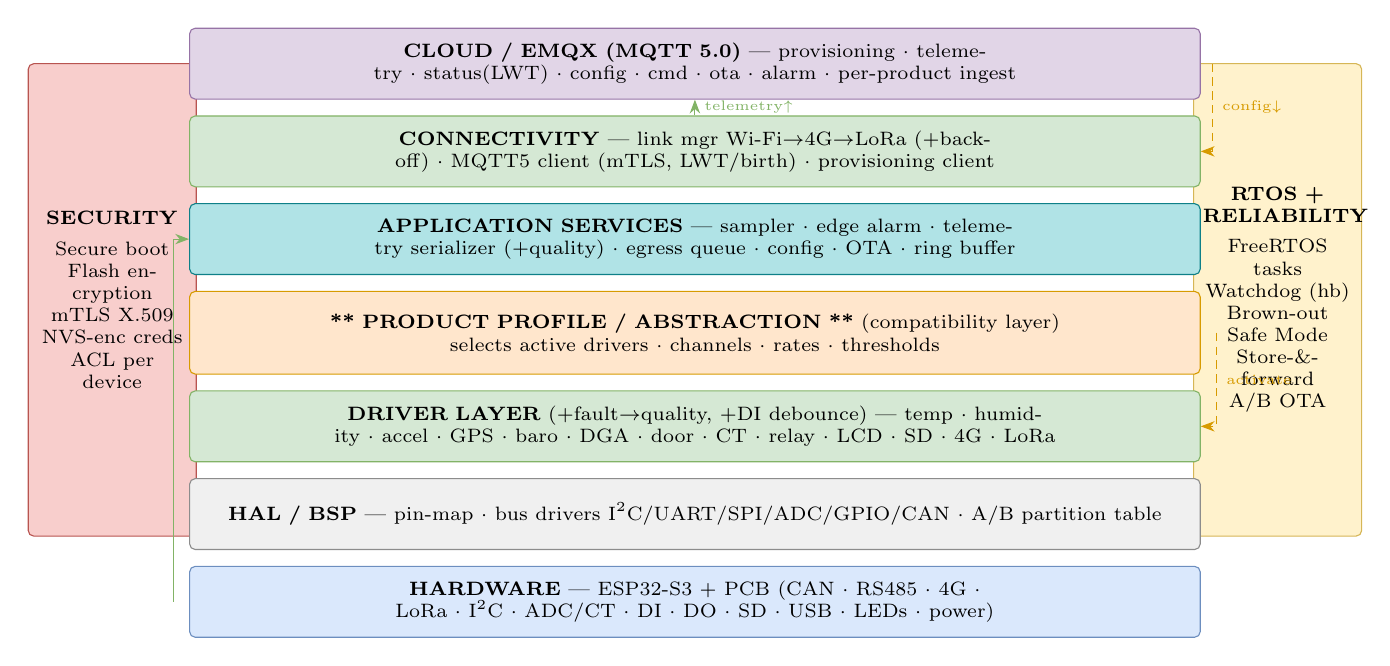
\begin{tikzpicture}
  \def\W{12.6cm}
  \node[sidebar={crossCol}{crossEdge}, minimum height=6.0cm] (sec) at (-7.4,-3.0)
    {\textbf{SECURITY}\\[3pt]Secure boot\\Flash encryption\\mTLS X.509\\NVS-enc creds\\ACL per device};
  \node[sidebar={sysCol}{sysEdge}, minimum height=6.0cm] (rt) at (7.4,-3.0)
    {\textbf{RTOS +}\\\textbf{RELIABILITY}\\[3pt]FreeRTOS tasks\\Watchdog (hb)\\Brown-out\\Safe Mode\\Store-\&-forward\\A/B OTA};
  \node[layer={cloudCol}{cloudEdge}{\W}] (l7) at (0,0)
    {\textbf{CLOUD / EMQX (MQTT 5.0)} — provisioning $\cdot$ telemetry $\cdot$ status(LWT) $\cdot$ config $\cdot$ cmd $\cdot$ ota $\cdot$ alarm $\cdot$ per-product ingest};
  \node[layer={drvCol}{drvEdge}{\W}, below=2mm of l7] (l6)
    {\textbf{CONNECTIVITY} — link mgr Wi-Fi$\to$4G$\to$LoRa (+backoff) $\cdot$ MQTT5 client (mTLS, LWT/birth) $\cdot$ provisioning client};
  \node[layer={appCol}{appEdge}{\W}, below=2mm of l6] (l5)
    {\textbf{APPLICATION SERVICES} — sampler $\cdot$ edge alarm $\cdot$ telemetry serializer (+quality) $\cdot$ egress queue $\cdot$ config $\cdot$ OTA $\cdot$ ring buffer};
  \node[layer={profCol}{profEdge}{\W}, below=2mm of l5, minimum height=1.05cm] (l4)
    {\textbf{** PRODUCT PROFILE / ABSTRACTION **} (compatibility layer)\\
     selects active drivers $\cdot$ channels $\cdot$ rates $\cdot$ thresholds};
  \node[layer={drvCol}{drvEdge}{\W}, below=2mm of l4] (l3)
    {\textbf{DRIVER LAYER} (+fault$\to$quality, +DI debounce) — temp $\cdot$ humidity $\cdot$ accel $\cdot$ GPS $\cdot$ baro $\cdot$ DGA $\cdot$ door $\cdot$ CT $\cdot$ relay $\cdot$ LCD $\cdot$ SD $\cdot$ 4G $\cdot$ LoRa};
  \node[layer={halCol}{halEdge}{\W}, below=2mm of l3] (l2)
    {\textbf{HAL / BSP} — pin-map $\cdot$ bus drivers I\textsuperscript{2}C/UART/SPI/ADC/GPIO/CAN $\cdot$ A/B partition table};
  \node[layer={hwCol}{hwEdge}{\W}, below=2mm of l2] (l1)
    {\textbf{HARDWARE} — ESP32-S3 + PCB (CAN $\cdot$ RS485 $\cdot$ 4G $\cdot$ LoRa $\cdot$ I\textsuperscript{2}C $\cdot$ ADC/CT $\cdot$ DI $\cdot$ DO $\cdot$ SD $\cdot$ USB $\cdot$ LEDs $\cdot$ power)};
  \draw[-{Stealth[length=5pt]}, drvEdge] (l1.west) ++(-0.2,0) |- (l5.west);
  \draw[-{Stealth[length=5pt]}, profEdge, densely dashed] (l4.east) ++(0.2,0) |- (l3.east)
        node[pos=0.25,right,font=\tiny]{activate};
  \draw[-{Stealth[length=5pt]}, drvEdge] (l6) -- (l7) node[midway,right,font=\tiny]{telemetry$\uparrow$};
  \draw[-{Stealth[length=5pt]}, profEdge, densely dashed] (l7.east) ++(0.15,0) |- (l6.east)
        node[pos=0.25,right,font=\tiny]{config$\downarrow$};
\end{tikzpicture}}
\caption{Layered firmware architecture; the highlighted product-profile layer is what makes one
image serve three products.}
\end{figure}

\section*{13\quad Boot \& provisioning flow}
The happy path is gated by fault checks: a hardware self-test can divert to Safe Mode, and
provisioning / link bring-up retry with \textbf{exponential backoff (cap + jitter)} so the flow
never reaches \texttt{MQTT connect} without a link layer.

\begin{figure}[H]
\centering
\resizebox{0.95\textwidth}{!}{%
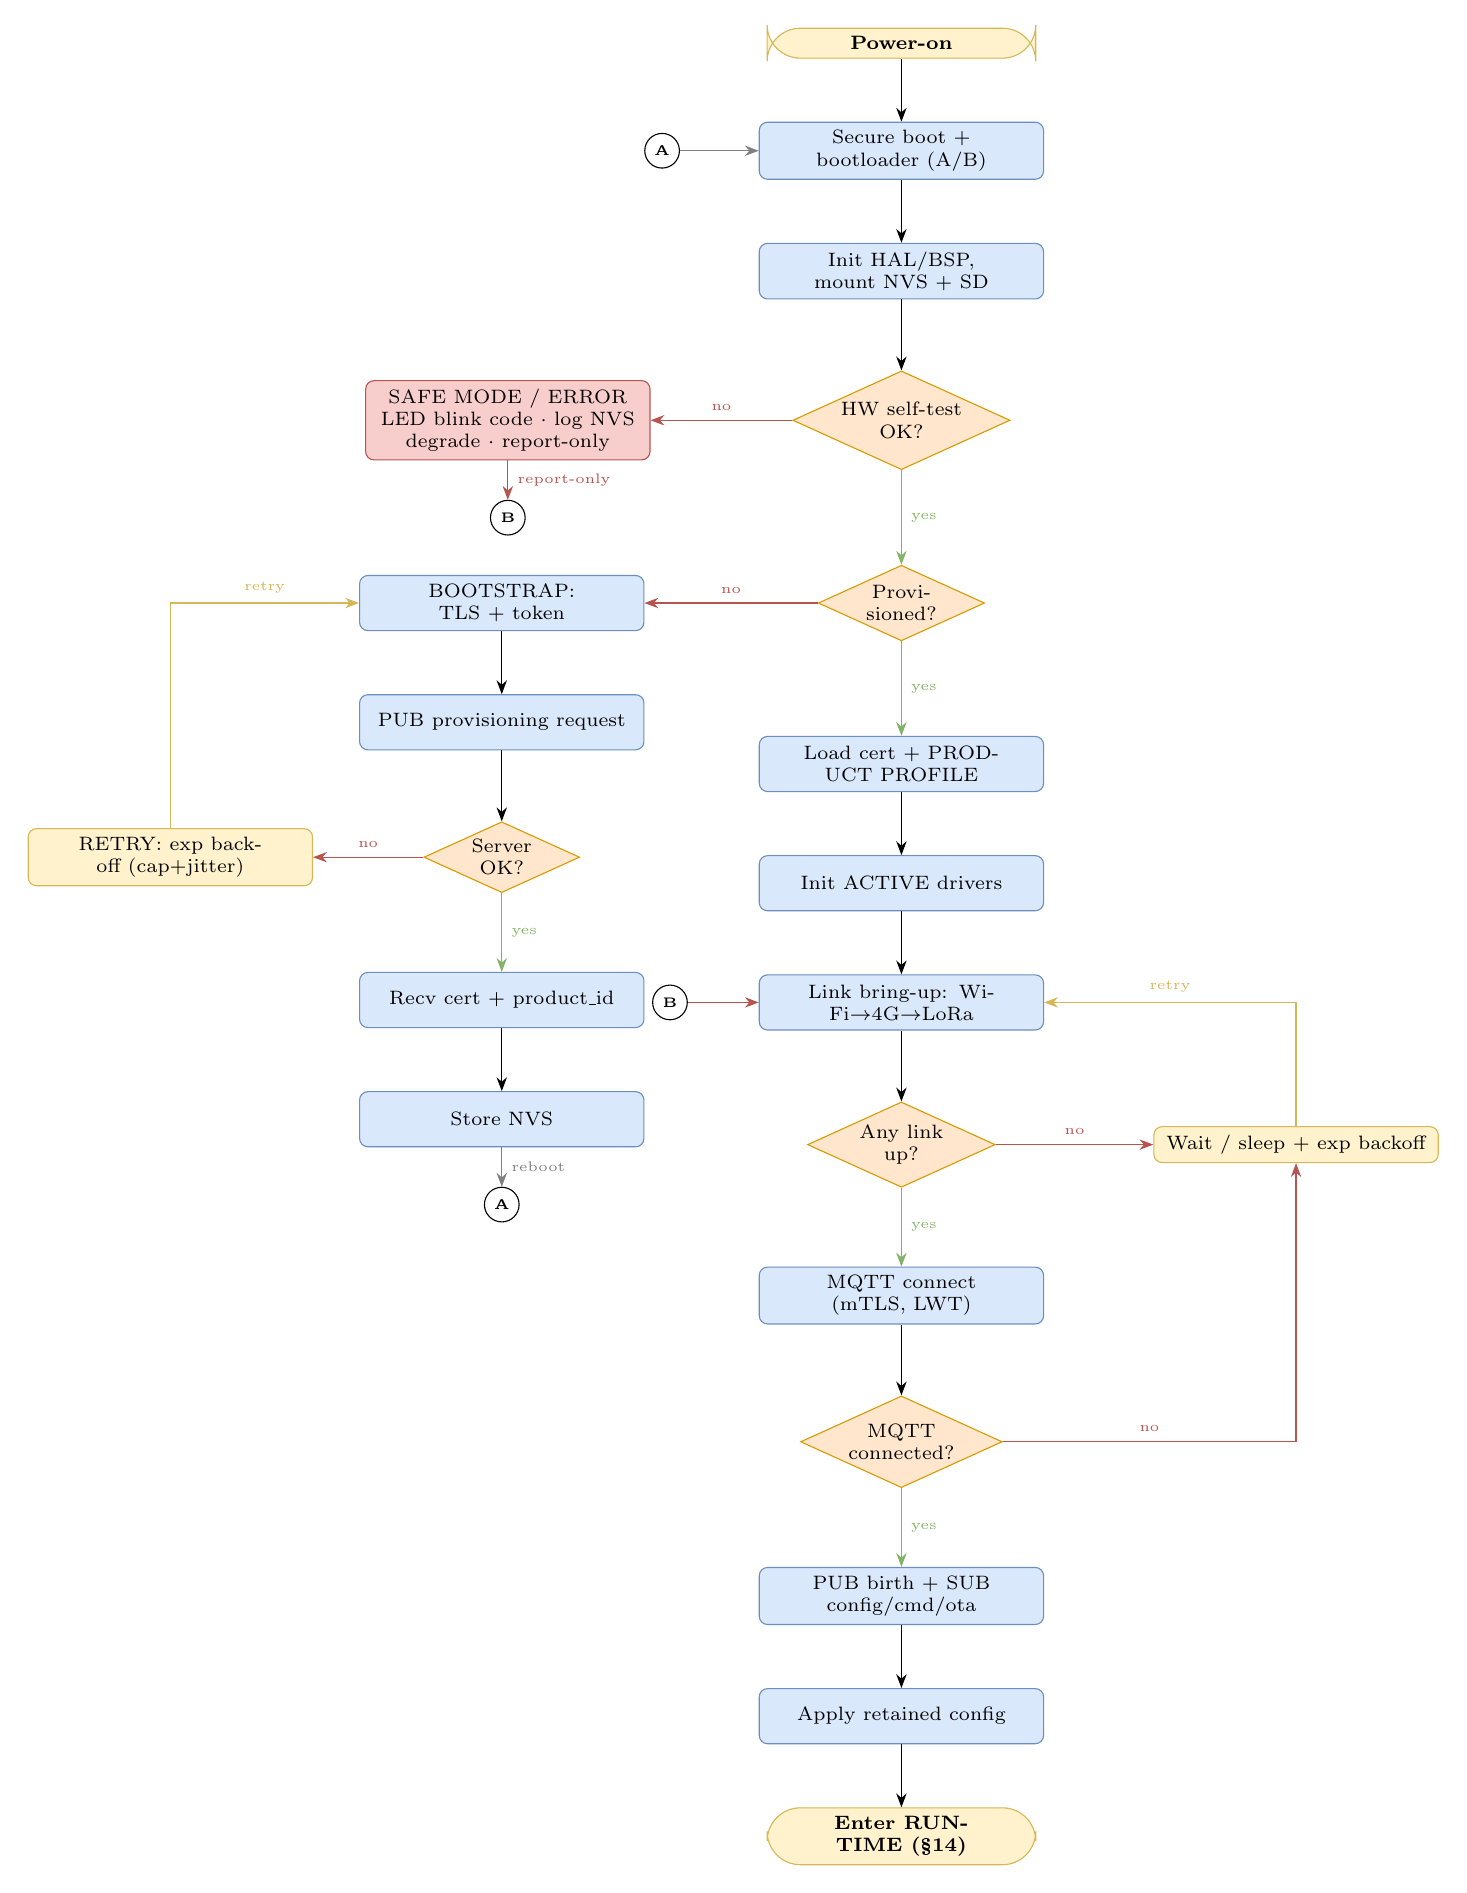
\begin{tikzpicture}[node distance=8mm and 10mm]
  \node[fterm] (s0) {Power-on};
  \node[fproc, below=of s0] (s1) {Secure boot + bootloader (A/B)};
  \node[fproc, below=of s1] (s2) {Init HAL/BSP, mount NVS + SD};
  \node[fdec, below=9mm of s2] (d1) {HW self-test\\OK?};
  \node[fsafe, left=18mm of d1] (safe) {SAFE MODE / ERROR\\LED blink code $\cdot$ log NVS\\degrade $\cdot$ report-only};
  \node[fdec, below=12mm of d1] (d2) {Provi-\\sioned?};
  % bootstrap branch (left)
  \node[fproc, left=22mm of d2] (b1) {BOOTSTRAP: TLS + token};
  \node[fproc, below=of b1] (b2) {PUB provisioning request};
  \node[fdec, below=9mm of b2] (d3) {Server\\OK?};
  \node[fback, left=14mm of d3] (bk1) {RETRY: exp backoff (cap+jitter)};
  \node[fproc, below=10mm of d3] (b3) {Recv cert + product\_id};
  \node[fproc, below=of b3] (b4) {Store NVS};
  % main spine (down)
  \node[fproc, below=12mm of d2] (m1) {Load cert + PRODUCT PROFILE};
  \node[fproc, below=of m1] (m2) {Init ACTIVE drivers};
  \node[fproc, below=of m2] (m3) {Link bring-up: Wi-Fi$\to$4G$\to$LoRa};
  \node[fdec, below=9mm of m3] (d4) {Any link\\up?};
  \node[fback, right=20mm of d4] (bk2) {Wait / sleep + exp backoff};
  \node[fproc, below=10mm of d4] (m4) {MQTT connect (mTLS, LWT)};
  \node[fdec, below=9mm of m4] (d5) {MQTT\\connected?};
  \node[fproc, below=10mm of d5] (m5) {PUB birth + SUB config/cmd/ota};
  \node[fproc, below=of m5] (m6) {Apply retained config};
  \node[fterm, below=of m6] (m7) {Enter RUNTIME (\S14)};
  % edges
  \tikzset{a/.style={-{Stealth[length=5pt]}, font=\tiny},
           conn/.style={draw, circle, fill=white, inner sep=0.6pt, font=\tiny\bfseries, minimum size=4.4mm}}
  \draw[a] (s0)--(s1); \draw[a] (s1)--(s2); \draw[a] (s2)--(d1);
  \draw[a,crossEdge] (d1)--(safe) node[midway,above,font=\tiny]{no};
  \draw[a,drvEdge] (d1)--(d2) node[midway,right,font=\tiny]{yes};
  \draw[a,crossEdge] (d2)--(b1) node[midway,above,font=\tiny]{no};
  \draw[a,drvEdge] (d2)--(m1) node[midway,right,font=\tiny]{yes};
  \draw[a] (b1)--(b2); \draw[a] (b2)--(d3);
  \draw[a,crossEdge] (d3)--(bk1) node[midway,above,font=\tiny]{no};
  \draw[a,sysEdge] (bk1.north) |- (b1.west) node[pos=0.75,above,font=\tiny]{retry};
  \draw[a,drvEdge] (d3)--(b3) node[midway,right,font=\tiny]{yes};
  \draw[a] (b3)--(b4);
  \draw[a] (m1)--(m2); \draw[a] (m2)--(m3); \draw[a] (m3)--(d4);
  \draw[a,crossEdge] (d4)--(bk2) node[midway,above,font=\tiny]{no};
  \draw[a,sysEdge] (bk2.north) |- (m3.east) node[pos=0.75,above,font=\tiny]{retry};
  \draw[a,drvEdge] (d4)--(m4) node[midway,right,font=\tiny]{yes};
  \draw[a] (m4)--(d5);
  \draw[a,crossEdge] (d5.east) -| (bk2.south) node[pos=0.25,above,font=\tiny]{no};
  \draw[a,drvEdge] (d5)--(m5) node[midway,right,font=\tiny]{yes};
  \draw[a] (m5)--(m6); \draw[a] (m6)--(m7);
  % on-page connectors (avoid spaghetti back-edges)
  \node[conn, below=5mm of b4] (jA){A};
  \draw[a,gray] (b4)--(jA) node[midway,right,font=\tiny]{reboot};
  \node[conn, left=10mm of s1] (jAr){A};
  \draw[a,gray] (jAr)--(s1.west);
  \node[conn, below=5mm of safe] (jB){B};
  \draw[a,crossEdge] (safe)--(jB) node[midway,right,font=\tiny]{report-only};
  \node[conn, left=9mm of m3] (jBr){B};
  \draw[a,crossEdge] (jBr)--(m3.west);
\end{tikzpicture}}
\caption{Boot \& provisioning with Safe-Mode diversion, bootstrap retry, and link/MQTT backoff
loops. Circled \textbf{A}/\textbf{B} are on-page connectors (jump to the same-letter target).}
\end{figure}

\section*{14\quad Runtime tasks \& data flow}
Sensor and alarm tasks never call publish directly. They enqueue to a single priority
\textbf{egress queue}; \texttt{LinkMgr} is the only publisher (drains one at a time, Alarm
QoS\,1 before Telemetry), which avoids MQTT-client races and lets the broker absorb back-pressure.

\begin{figure}[H]
\centering
\resizebox{\textwidth}{!}{%
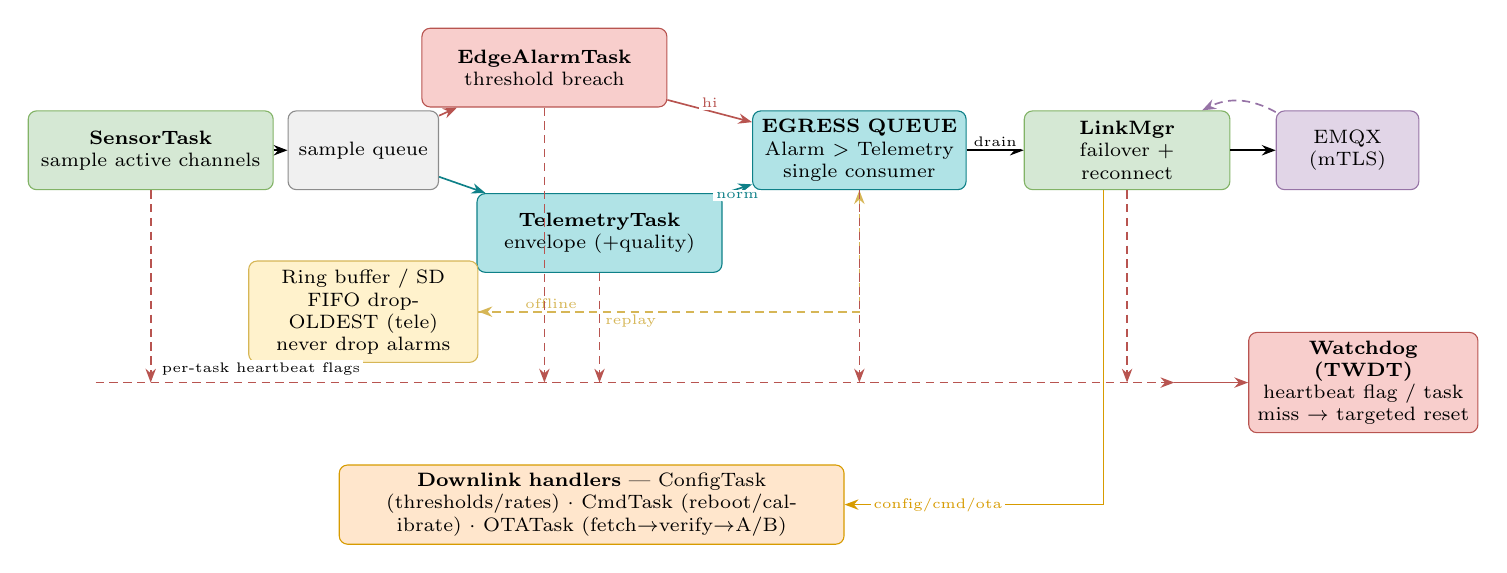
\begin{tikzpicture}
  \tikzset{tk/.style n args={2}{draw=#2, fill=#1, rounded corners=3pt, align=center,
        font=\scriptsize, inner sep=3pt, text width=2.9cm, minimum height=1.0cm}}
  % --- uplink pipeline ---
  \node[tk={drvCol}{drvEdge}] (sens) at (0,0) {\textbf{SensorTask}\\sample active channels};
  \node[tk={halCol}{halEdge}, text width=1.7cm] (q1) at (2.7,0) {sample queue};
  \node[tk={crossCol}{crossEdge}] (al) at (5.0,1.05) {\textbf{EdgeAlarmTask}\\threshold breach};
  \node[tk={appCol}{appEdge}] (te) at (5.7,-1.05) {\textbf{TelemetryTask}\\envelope (+quality)};
  \node[tk={appCol}{appEdge}, text width=2.5cm] (eg) at (9.0,0)
       {\textbf{EGRESS QUEUE}\\Alarm $>$ Telemetry\\single consumer};
  \node[tk={drvCol}{drvEdge}, text width=2.4cm] (link) at (12.4,0) {\textbf{LinkMgr}\\failover + reconnect};
  \node[tk={cloudCol}{cloudEdge}, text width=1.6cm] (br) at (15.2,0) {EMQX\\(mTLS)};
  \node[tk={sysCol}{sysEdge}, text width=2.7cm] (buf) at (2.7,-2.05)
       {Ring buffer / SD\\FIFO drop-OLDEST (tele)\\never drop alarms};
  % --- downlink handlers + watchdog ---
  \node[tk={profCol}{profEdge}, text width=6.2cm] (dl) at (5.6,-4.5)
       {\textbf{Downlink handlers} — ConfigTask (thresholds/rates) $\cdot$ CmdTask (reboot/calibrate) $\cdot$ OTATask (fetch$\to$verify$\to$A/B)};
  \node[tk={crossCol}{crossEdge}, text width=2.7cm] (wdt) at (15.4,-2.95)
       {\textbf{Watchdog (TWDT)}\\heartbeat flag / task\\miss $\to$ targeted reset};
  % uplink edges
  \draw[flow] (sens)--(q1);
  \draw[flow,crossEdge] (q1)--(al); \draw[flow,appEdge] (q1)--(te);
  \draw[flow,crossEdge] (al)--(eg) node[elab,pos=0.5,above]{hi};
  \draw[flow,appEdge] (te)--(eg) node[elab,pos=0.5,below]{norm};
  \draw[flow] (eg)--(link) node[elab,midway,above]{drain};
  \draw[flow] (link)--(br);
  % store-and-forward
  \draw[flowd,sysEdge] (te.south) |- (buf.east) node[elab,pos=0.7,above]{offline};
  \draw[flowd,sysEdge] (buf.east) -| (eg.south) node[elab,pos=0.2,below]{replay};
  % downlink: broker -> link -> handlers
  \draw[flowd,cloudEdge] (br) to[bend right=28] (link);
  \draw[flow,profEdge] ([xshift=-3mm]link.south) |- (dl.east) node[elab,pos=0.82]{config/cmd/ota};
  % heartbeat bus -> watchdog
  \draw[flowd,crossEdge] (-0.7,-2.95) -- (13.0,-2.95);
  \node[font=\tiny, fill=white, inner sep=1pt] at (1.4,-2.78){per-task heartbeat flags};
  \foreach \t in {sens,al,te,eg,link} \draw[flowd,crossEdge] (\t.south) -- (\t.south|-0,-2.95);
  \draw[flow,crossEdge] (13.0,-2.95)--(wdt.west);
\end{tikzpicture}}
\caption{Runtime FreeRTOS tasks, priority egress queue, store-and-forward, downlink handlers and
heartbeat watchdog.}
\end{figure}

\section*{15\quad Link Manager state machine}
The FSM below governs the \emph{state} of the active link; \emph{which} transport to select and
the anti-flapping rule that prevents needless switching are specified in \S21.
\begin{figure}[H]
\centering
\resizebox{0.96\textwidth}{!}{%
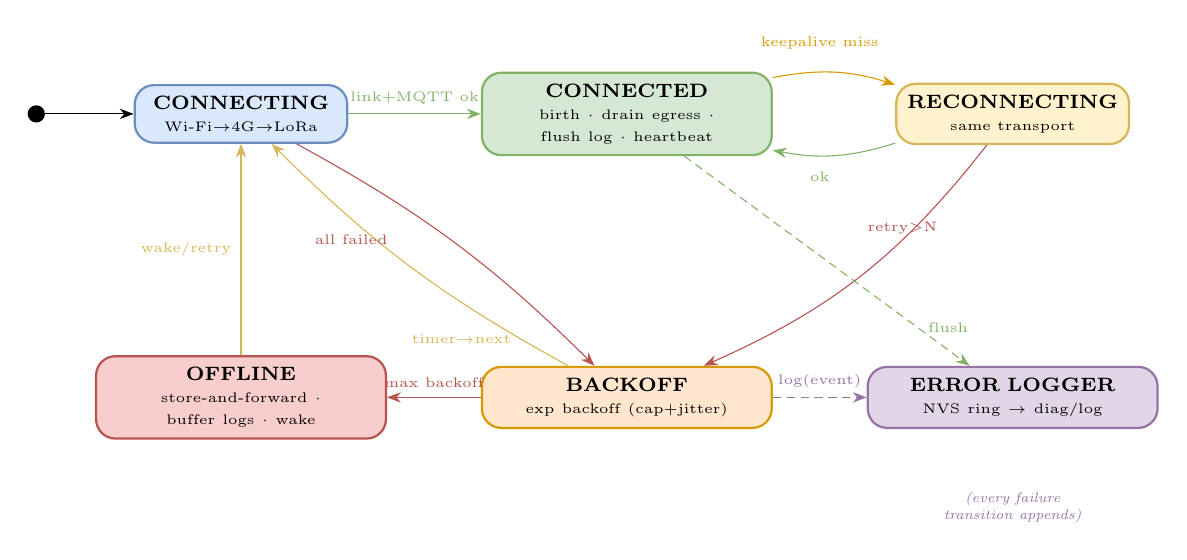
\begin{tikzpicture}
  \node[circle, fill=black, inner sep=2.2pt] (i) at (-6.0,2.3){};
  \node[stnode={hwCol}{hwEdge}] (cn) at (-3.4,2.3){\textbf{CONNECTING}\\\tiny Wi-Fi$\to$4G$\to$LoRa};
  \node[stnode={drvCol}{drvEdge}, text width=3.4cm] (co) at (1.5,2.3)
       {\textbf{CONNECTED}\\\tiny birth $\cdot$ drain egress $\cdot$ flush log $\cdot$ heartbeat};
  \node[stnode={sysCol}{sysEdge}] (rc) at (6.4,2.3){\textbf{RECONNECTING}\\\tiny same transport};
  \node[stnode={crossCol}{crossEdge}, text width=3.4cm] (of) at (-3.4,-1.3)
       {\textbf{OFFLINE}\\\tiny store-and-forward $\cdot$ buffer logs $\cdot$ wake};
  \node[stnode={profCol}{profEdge}, text width=3.4cm] (bk) at (1.5,-1.3)
       {\textbf{BACKOFF}\\\tiny exp backoff (cap+jitter)};
  \node[stnode={cloudCol}{cloudEdge}, text width=3.4cm] (lg) at (6.4,-1.3)
       {\textbf{ERROR LOGGER}\\\tiny NVS ring $\to$ diag/log};
  \tikzset{t/.style={-{Stealth[length=5pt]}, font=\tiny}}
  \draw[t] (i)--(cn);
  \draw[t,drvEdge] (cn)--(co) node[midway,above,font=\tiny]{link+MQTT ok};
  \draw[t,profEdge] (co) to[bend left=14] (rc);
  \draw[t,drvEdge] (rc) to[bend left=14] (co);
  \draw[t,crossEdge] (cn) to[bend left=8] (bk);
  \draw[t,crossEdge] (rc) to[bend left=14] (bk);
  \draw[t,sysEdge] (bk) to[bend left=8] (cn);
  \draw[t,crossEdge] (bk)--(of) node[midway,above,font=\tiny]{max backoff};
  \draw[t,sysEdge] (of)--(cn) node[midway,left,font=\tiny]{wake/retry};
  % logging (kept minimal: flush on CONNECTED, append on failure)
  \draw[t,drvEdge,densely dashed] (co)--(lg) node[pos=0.82,right,font=\tiny]{flush};
  \draw[t,cloudEdge,densely dashed] (bk)--(lg) node[midway,above,font=\tiny]{log(event)};
  % explicitly-placed transition labels (no central pile-up)
  \node[font=\tiny, text=profEdge]  at (3.95,3.2){keepalive miss};
  \node[font=\tiny, text=drvEdge]   at (3.95,1.5){ok};
  \node[font=\tiny, text=crossEdge] at (-2.0,0.7){all failed};
  \node[font=\tiny, text=sysEdge]   at (-0.6,-0.55){timer$\to$next};
  \node[font=\tiny, text=crossEdge] at (5.0,0.85){retry$>$N};
  \node[font=\tiny\itshape, text=cloudEdge, align=center] at (6.4,-2.7){(every failure\\transition appends)};
\end{tikzpicture}}
\caption{Link Manager FSM: transport failover, backoff, and an error logger that flushes the NVS
ring to \texttt{diag/log} when CONNECTED (so offline faults still reach the cloud).}
\end{figure}

\section*{16\quad Diagnostics: \texttt{diag/log} schema \& codes}
Topic \texttt{\{tenant\}/\{product\}/\{device\}/diag/log} $\cdot$ QoS\,1 $\cdot$ retain=0 $\cdot$ batched flush.

\begin{lstlisting}[style=js]
{
  "v": 1,                       // schema version
  "device_id": "ac-fridge-0042",
  "tenant": "acme", "product": "carbonbox",   // eternity|carbonbox|bloodbox
  "fw": "1.4.2",
  "boot_id": 137,               // ++ each boot (detect resets)
  "sent_at": 1733740800000,     // wall clock at flush (epoch ms)
  "uptime_s": 86230,
  "dropped": 4,                 // entries lost to ring overflow
  "events": [
    { "seq": 5012,              // monotonic per device (gap/dedupe)
      "t": 1733740123000,       // epoch ms, or null if pre-time-sync
      "up": 85553,              // uptime_s when logged (ALWAYS set)
      "time_src": "rtc",        // ntp|lorawan|rtc|uptime  (see 10.1)
      "lvl": "warn",            // info|warn|err|fatal
      "code": "LINK_KEEPALIVE_MISS",
      "from": "CONNECTED", "to": "RECONNECTING",
      "tr": "wifi", "rssi": -78,
      "msg": "3 keepalives missed",
      "ctx": { "heap": 142000, "retries": 0 } }
  ]
}
\end{lstlisting}
\noindent\textbf{Notes.} Batched on entering CONNECTED; \texttt{t} now comes from the RTC even
offline (\S10.1) — \texttt{time\_src} records which clock stamped it; \texttt{t=null} only on the
rare pre-RTC boot race, where \texttt{up} still lets ingest reconstruct wall time as
\texttt{sent\_at\,$-$\,(uptime\_s\,$-$\,up)}; \texttt{seq} gives gap detection; alarms are
\emph{not} sent here (they use \texttt{\dots /alarm/\{sid\}}).

\begin{center}
\renewcommand{\arraystretch}{1.1}\footnotesize
\begin{tabularx}{\textwidth}{@{}l l l X@{}}
\toprule
\textbf{code} & \textbf{lvl} & \textbf{LED blink} & \textbf{meaning} \\
\midrule
\texttt{HW\_SD\_FAIL} & err & 2$\times$ long & SD mount/format failed \\
\texttt{HW\_I2C\_TIMEOUT} & err & 3$\times$ long & I\textsuperscript{2}C bus stuck $\to$ recover \\
\texttt{SENSOR\_OPEN\_WIRE} & warn & 2$\times$ short & open/loose $\to$ \texttt{quality=error} \\
\texttt{SENSOR\_I2C\_NACK} & warn & 2$\times$ short & no ACK $\to$ \texttt{quality=error} \\
\texttt{SENSOR\_STALE} & warn & --- & no fresh read $\to$ \texttt{quality=stale} \\
\texttt{PROV\_TOKEN\_FAIL} & err & 4$\times$ long & factory token rejected \\
\texttt{LINK\_ALL\_FAILED} & err & 1\,Hz & Wi-Fi+4G+LoRa all down \\
\texttt{LINK\_KEEPALIVE\_MISS} & warn & --- & $\to$ RECONNECTING \\
\texttt{LINK\_OFFLINE} & err & 1\,Hz & store-and-forward active \\
\texttt{LINK\_RESTORED} & info & --- & CONNECTED, flushing log \\
\texttt{BUF\_OVERFLOW\_DROP} & warn & --- & ring full $\to$ drop oldest \\
\texttt{OTA\_VERIFY\_FAIL} & err & 5$\times$ short & SHA / secure-boot mismatch \\
\texttt{OTA\_ROLLBACK} & err & 5$\times$ short & A/B partition reverted \\
\texttt{WDT\_RESET} & fatal & solid & task hang $\to$ targeted reset \\
\texttt{BROWNOUT} & fatal & solid & power-dip reset \\
\bottomrule
\end{tabularx}
\end{center}

\section*{17\quad Robustness \& fault-handling summary}
\begin{itemize}[leftmargin=1.4em,itemsep=1pt]
  \item \textbf{Safe Mode} on HW self-test failure (SD/I\textsuperscript{2}C/power): LED error code, NVS fault log,
        skip the faulty subsystem, attempt a report-only link — never hang.
  \item \textbf{Exponential backoff (cap + jitter)} on bootstrap, link bring-up and MQTT connect;
        a link-fallback loop guarantees the flow never enters \texttt{MQTT connect} without a link.
  \item \textbf{Priority egress queue} (Alarm QoS\,1 > Telemetry) with \texttt{LinkMgr} as sole
        publisher; \textbf{ring buffer} policy is FIFO drop-oldest for telemetry, never for alarms.
  \item \textbf{Watchdog} via per-task heartbeat flags $\to$ targeted reset of the hung task.
  \item \textbf{Sensor faults} surface as \texttt{quality=error:<code>} (never a false \texttt{0});
        \textbf{digital inputs} are debounced/rate-limited in the ISR.
  \item \textbf{Diagnostics} (\texttt{diag/log}) are flushed when CONNECTED so offline faults still
        reach the cloud; alarms stay on their own topic.
\end{itemize}

% =====================================================================
\newpage
\section*{18\quad LoRaWAN integration \& provisioning}
On Wi-Fi / 4G the device speaks MQTT/mTLS to EMQX \emph{directly} (Part~I, Phase~A). Over LoRaWAN
it cannot: the ESP32 transmits compact binary frames to a \textbf{LoRa gateway}; a
\textbf{LoRaWAN Network Server (LNS)} — ChirpStack or The Things Network — terminates the LoRaWAN
MAC, runs the OTAA join, de-duplicates and decrypts, then \textbf{bridges} decoded uplinks into the
\emph{same} EMQX topic namespace. On-air confidentiality is LoRaWAN AES-128 (NwkSKey/AppSKey), not mTLS.

\begin{figure}[H]
\centering
\resizebox{\textwidth}{!}{%
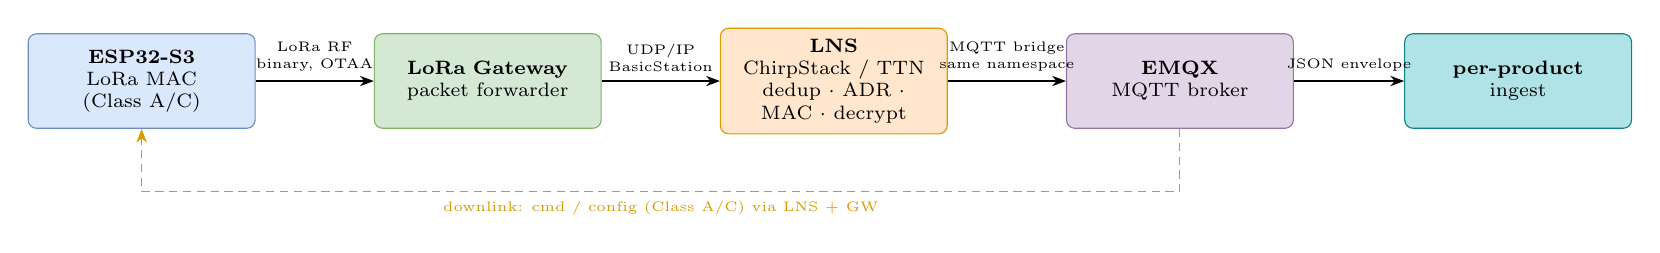
\begin{tikzpicture}[every node/.style={font=\scriptsize}]
  \tikzset{bx/.style n args={2}{draw=#2,fill=#1,rounded corners=3pt,align=center,inner sep=4pt,
        minimum height=1.2cm,text width=2.6cm}}
  \node[bx={hwCol}{hwEdge}] (dev){\textbf{ESP32-S3}\\LoRa MAC\\(Class A/C)};
  \node[bx={drvCol}{drvEdge}, right=1.5cm of dev] (gw){\textbf{LoRa Gateway}\\packet forwarder};
  \node[bx={profCol}{profEdge}, right=1.5cm of gw] (lns){\textbf{LNS}\\ChirpStack / TTN\\dedup $\cdot$ ADR $\cdot$ MAC $\cdot$ decrypt};
  \node[bx={cloudCol}{cloudEdge}, right=1.5cm of lns] (emqx){\textbf{EMQX}\\MQTT broker};
  \node[bx={appCol}{appEdge}, right=1.4cm of emqx] (ing){\textbf{per-product}\\ingest};
  \draw[-{Stealth[length=5pt]}] (dev)--(gw) node[midway,above,font=\tiny,align=center]{LoRa RF\\binary, OTAA};
  \draw[-{Stealth[length=5pt]}] (gw)--(lns) node[midway,above,font=\tiny,align=center]{UDP/IP\\BasicStation};
  \draw[-{Stealth[length=5pt]}] (lns)--(emqx) node[midway,above,font=\tiny,align=center]{MQTT bridge\\same namespace};
  \draw[-{Stealth[length=5pt]}] (emqx)--(ing) node[midway,above,font=\tiny]{JSON envelope};
  \draw[-{Stealth[length=5pt]},densely dashed,profEdge] (emqx.south) -- ++(0,-0.8) -| (dev.south)
        node[pos=0.25,below,font=\tiny]{downlink: cmd / config (Class A/C) via LNS + GW};
\end{tikzpicture}}
\caption{LoRaWAN data path. The gateway + LNS replace the direct MQTT/mTLS hop; the LNS bridge
re-publishes decoded frames under \texttt{\{tenant\}/\{product\}/\{device\}/\dots} so the cloud
side (ingest, alarm engine) is transport-agnostic.}
\end{figure}

\paragraph{OTAA credentials (injected at End-of-Line, \S19).}
\begin{center}
\renewcommand{\arraystretch}{1.22}\small
\begin{tabularx}{\textwidth}{@{}l l l X@{}}
\toprule
\textbf{Credential} & \textbf{Source (factory)} & \textbf{Stored} & \textbf{Role} \\
\midrule
\texttt{DevEUI} & chip base-MAC or assigned & eFuse/NVS + label & globally-unique device id on air \\
\texttt{JoinEUI} (AppEUI) & tenant / application id & encrypted NVS & routes the join to the right join-server \\
\texttt{AppKey} (root) & per-device, generated at EOL & encrypted NVS (never leaves) + LNS & derives session keys at join \\
\bottomrule
\end{tabularx}
\end{center}
\noindent\textbf{Join (OTAA):} \texttt{JoinRequest(DevEUI, JoinEUI, DevNonce)} $\to$
\texttt{JoinAccept} $\to$ device derives \texttt{NwkSKey}, \texttt{AppSKey}, \texttt{DevAddr}. The
\texttt{AppKey} and the mTLS certificate are injected \emph{together} at EOL, so one device carries
credentials for both transports.

\paragraph{Binary payload (FPort-multiplexed).}
A LoRaWAN frame is tiny (EU868: $\approx$51\,B at DR0 up to 222\,B at DR5), so JSON is impossible.
Active channels are \textbf{batched} into one compact frame; the LNS decoder (or an EMQX rule)
re-expands them into the per-channel canonical envelope — this reconciles the ``one PUB per channel''
of Part~I, which applies only on IP transports.
\begin{center}
\renewcommand{\arraystretch}{1.18}\small
\begin{tabularx}{\textwidth}{@{}c l c l l X@{}}
\toprule
\textbf{FPort} & \textbf{Message} & \textbf{Dir} & \textbf{Codec} & \textbf{Size} & \textbf{Notes} \\
\midrule
1  & telemetry batch (active channels) & up   & CBOR / packed C-struct & 8--30\,B & per-product channel set \\
2  & heartbeat                         & up   & C-struct               & 6\,B     & rssi, batt, fw \\
3  & edge alarm                        & up   & C-struct               & 5\,B     & high priority, confirmed up \\
10 & \texttt{diag/log} (compact)        & up   & CBOR                   & 12--40\,B& subset of \S16 \\
20 & cmd (reboot/calibrate/threshold)  & down & C-struct               & 4--12\,B & Class A/C \\
21 & config delta (thresholds/rates)   & down & CBOR                   & 8--40\,B & not full \texttt{config} \\
\bottomrule
\end{tabularx}
\end{center}
\noindent\textbf{Recommendation:} \textbf{CBOR} for schema-evolvable messages (telemetry, diag,
config) and a \textbf{versioned C-struct} (first byte = schema version) for the fixed,
size-critical ones (heartbeat, alarm). \textbf{Full OTA images are never sent over LoRa} (use
Wi-Fi/4G, \S\,Phase~C); only small config/threshold pushes go down FPort\,21.

% =====================================================================
\newpage
\section*{19\quad End-of-Line (EOL) manufacturing \& silicon provisioning}
\texttt{eFuse} burning is \textbf{one-time and irreversible} — a wrong key bricks the chip. The line
therefore generates secrets \emph{on-chip}, tests \emph{first}, and burns fuses \emph{last}.

\begin{figure}[H]
\centering
\resizebox{\textwidth}{!}{%
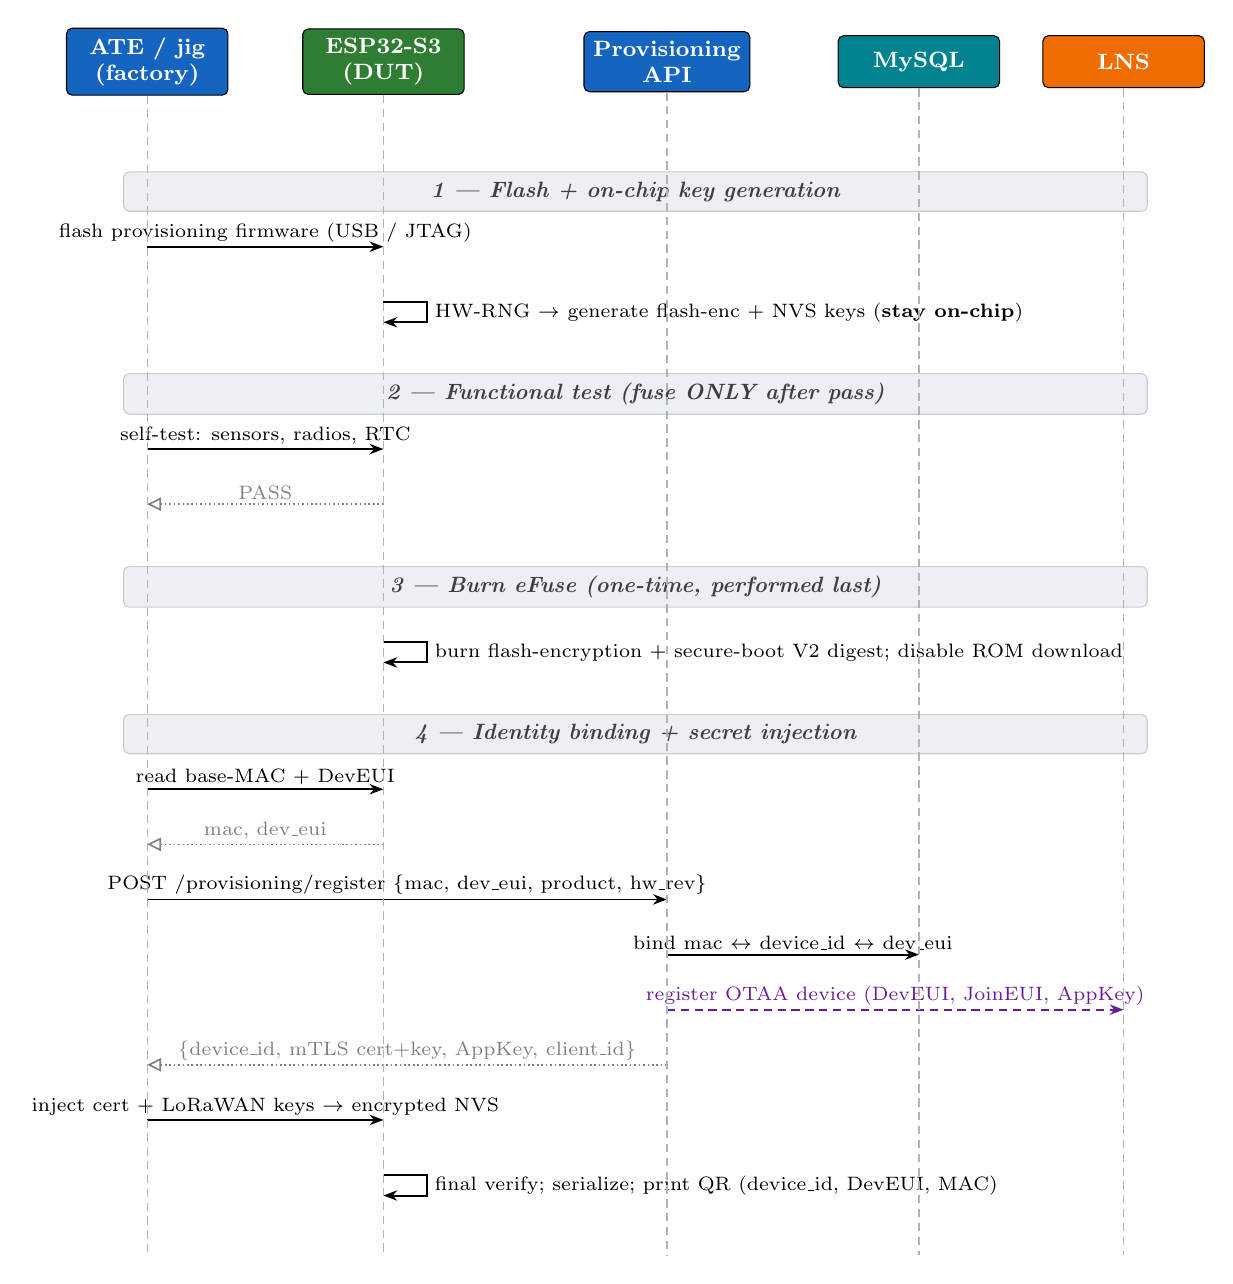
\begin{tikzpicture}
  \def\A{0}\def\D{3.0}\def\P{6.6}\def\M{9.8}\def\L{12.4}
  \def\xmid{6.2}\def\bandw{13.0cm}
  \seqreset
  \node[head, fill=svcCol] (p0) at (\A,0) {ATE / jig\\(factory)};
  \node[head, fill=devCol] (p1) at (\D,0) {ESP32-S3\\(DUT)};
  \node[head, fill=svcCol] (p2) at (\P,0) {Provisioning\\API};
  \node[head, fill=dbCol]  (p3) at (\M,0) {MySQL};
  \node[head, fill=otaCol] (p4) at (\L,0) {LNS};

  \phase{1 — Flash + on-chip key generation}
  \mO{\A}{\D}{flash provisioning firmware (USB / JTAG)}
  \mS{\D}{HW-RNG $\to$ generate flash-enc + NVS keys (\textbf{stay on-chip})}

  \phase{2 — Functional test (fuse ONLY after pass)}
  \mO{\A}{\D}{self-test: sensors, radios, RTC}
  \mR{\D}{\A}{PASS}

  \phase{3 — Burn eFuse (one-time, performed last)}
  \mS{\D}{burn flash-encryption + secure-boot V2 digest; disable ROM download}

  \phase{4 — Identity binding + secret injection}
  \mO{\A}{\D}{read base-MAC + DevEUI}
  \mR{\D}{\A}{mac, dev\_eui}
  \mO{\A}{\P}{POST /provisioning/register \{mac, dev\_eui, product, hw\_rev\}}
  \mO{\P}{\M}{bind mac $\leftrightarrow$ device\_id $\leftrightarrow$ dev\_eui}
  \mA{\P}{\L}{register OTAA device (DevEUI, JoinEUI, AppKey)}
  \mR{\P}{\A}{\{device\_id, mTLS cert+key, AppKey, client\_id\}}
  \mO{\A}{\D}{inject cert + LoRaWAN keys $\to$ encrypted NVS}
  \mS{\D}{final verify; serialize; print QR (device\_id, DevEUI, MAC)}

  \pgfmathsetmacro{\YBOT}{\YY-0.2}
  \foreach \p in {p0,p1,p2,p3,p4}{\draw[lifeline] (\p.south) -- (\p.south|-0,\YBOT);}
\end{tikzpicture}}
\caption{EOL provisioning. Keys are born on the chip and never leave it; the ATE only moves the
\emph{public} identity (MAC, DevEUI) to the cloud and injects the per-device cert + LoRaWAN
\texttt{AppKey}. Fuses are burned after the functional test to minimise scrap.}
\end{figure}

\paragraph{MAC $\to$ \texttt{device\_id} binding API.} \texttt{POST /api/v1/provisioning/register}
returns \texttt{\{device\_id, tenant, mqtt\_client\_id, cert, app\_key\}} and writes the immutable
\texttt{(mac, dev\_eui, device\_id, product, hw\_rev)} tuple to the \texttt{devices} table — the same
row later joined by the ingest path. The cert CN is \texttt{\{tenant\}.\{product\}.\{device\}} (\S7).

\paragraph{eFuse safety.} Burning is irreversible: \textbf{(a)} dry-run and verify all key digests
before the burn; \textbf{(b)} burn as the \emph{last} step, only after every functional test passes;
\textbf{(c)} keep the secure-boot \emph{signing} key in an HSM — only its public digest is fused,
never on the production line.

% =====================================================================
\section*{20\quad Flash partition table (16\,MB, frozen at v1)}
The A/B OTA scheme requires \texttt{ota\_0} and \texttt{ota\_1} to be \emph{equal-sized}; changing any
app slot later breaks the bootloader's slot arithmetic. This table is therefore part of the spec, not
a per-build choice.
\begin{center}
\renewcommand{\arraystretch}{1.18}\small
\begin{tabularx}{\textwidth}{@{}l l l r X@{}}
\toprule
\textbf{Name} & \textbf{Type} & \textbf{SubType} & \textbf{Size} & \textbf{Purpose} \\
\midrule
\texttt{nvs\_keys} & data & nvs\_keys & 4\,KB & flash-encryption key store \\
\texttt{otadata}   & data & ota       & 8\,KB & A/B boot selector \\
\texttt{phy\_init} & data & phy       & 4\,KB & RF calibration \\
\texttt{nvs}       & data & nvs       & 1\,MB & mTLS cert, LoRaWAN keys, config \\
\texttt{factory}   & app  & factory   & 3\,MB & immutable golden-recovery image \\
\texttt{ota\_0}    & app  & ota\_0    & 3\,MB & OTA slot A \\
\texttt{ota\_1}    & app  & ota\_1    & 3\,MB & OTA slot B \\
\texttt{storage}   & data & littlefs  & $\approx$5.9\,MB & ring-buffer staging before SD \\
\bottomrule
\end{tabularx}
\end{center}
\begin{lstlisting}[style=js]
# ESP-IDF partitions-16MB.csv  (offsets auto; app partitions 64 KB-aligned)
# Name,     Type, SubType,  Size
nvs_keys,   data, nvs_keys, 0x1000
otadata,    data, ota,      0x2000
phy_init,   data, phy,      0x1000
nvs,        data, nvs,      0x100000
factory,    app,  factory,  0x300000
ota_0,      app,  ota_0,    0x300000
ota_1,      app,  ota_1,    0x300000
storage,    data, littlefs, 0x5F0000
\end{lstlisting}
\noindent If golden-recovery is not required, drop \texttt{factory} and grow \texttt{storage} by
3\,MB — but keep \texttt{ota\_0}\,=\,\texttt{ota\_1}.

% =====================================================================
\section*{21\quad Transport selection \& hysteresis (anti-flapping)}
The FSM (\S15) handles \emph{losing} a link; this section handles \emph{choosing} one without
chattering. Transports are ranked by bandwidth/cost; the device commits to one and resists switching
back up until the better link has proven stable — the link-layer analogue of the alarm 2-reading
debounce (\S8).
\begin{center}
\renewcommand{\arraystretch}{1.22}\small
\begin{tabularx}{\textwidth}{@{}l c c c X@{}}
\toprule
\textbf{Transport} & \textbf{Rank} & \textbf{Switch-up dwell} & \textbf{Switch-down} & \textbf{Notes} \\
\midrule
Wi-Fi      & 0 (preferred) & 20\,s & immediate on loss & cheapest, highest BW; full OTA here \\
4G / LTE   & 1             & 30\,s & immediate on loss & metered; full OTA here \\
LoRaWAN    & 2 (floor)     & ---   & n/a               & always-available fallback; binary only (\S18) \\
\bottomrule
\end{tabularx}
\end{center}
\begin{itemize}[leftmargin=1.4em,itemsep=1pt]
  \item \textbf{Switch-down} (to a lower rank) is \emph{immediate} on active-link loss — fast
        failover, exactly the \texttt{BACKOFF}/\texttt{OFFLINE} paths of \S15.
  \item \textbf{Switch-up} (back to a higher rank) only when that link has been \emph{continuously}
        healthy for its dwell time \emph{and} no publish is in flight. Each link keeps a
        \texttt{stable\_since}; the guard is \texttt{now $-$ stable\_since $\geq$ dwell}.
  \item This stops a BloodBOX in transit through patchy 4G from flapping Wi-Fi/4G/LoRa every few
        seconds and burning power + bandwidth on repeated mTLS handshakes.
  \item The link being \emph{left} still carries the \S15 exponential backoff, so a marginal link is
        not re-probed faster than its backoff allows.
\end{itemize}


\end{document}
